\documentclass[a4paper, 12pt, oneside, titlepage, BCOR=1mm, DIV=12]{article}
\usepackage[a4paper,top=2cm,bottom=2cm,left=1cm,right=1cm]{geometry}

\usepackage[utf8]{inputenc}
\usepackage[english,ukrainian]{babel}
\usepackage[document]{ragged2e}
\usepackage{fancyhdr}
\usepackage{mathtext}
\usepackage{scrextend}
\usepackage{eqnarray,amsmath,amssymb}
\usepackage{color}
\usepackage{setspace}
\usepackage{graphicx}
\usepackage{hyperref}

\newcommand{\Lim}[1]{\raisebox{0.5ex}{{$\displaystyle \lim_{#1}\;$}}}
\newcommand{\Sum}[2]{\raisebox{0.5ex}{{$\displaystyle \sum_{#1}^{#2}\;$}}}


% checkboxes! щоб перевіряти чи правильно

\renewcommand{\d}[1]{
  \hspace{2pt}\text{d}\hspace{1pt}{#1}
}

\newcommand{\dx}{\hspace{2pt}\text{ERRROR}}
\newcommand{\dt}{\hspace{2pt}\text{ERRROR}}
\newcommand{\du}{\hspace{2pt}\text{ERRROR}}
\newcommand{\dv}{\hspace{2pt}\text{ERRROR}}
\newcommand{\dw}{\hspace{2pt}\text{ERRROR}}

\definecolor{orange}{RGB}{255,65,0}
\definecolor{red}{RGB}{255,0,0}
\definecolor{gray}{RGB}{190,190,190}
\definecolor{green}{RGB}{0,128,0}
% \definecolor{green}{RGB}{0,0,0} % pre production value

\newcommand{\task}[2]{
  % pre print option
  \framebox[4cm]{ \par $\square$ {\color{#1}#2} }
  % e-paper check boxes
  % \framebox[4cm]{ \par \hspace*{-.3cm}{\CheckBox[width=10pt,height=10pt,bordercolor=0 0 0,name=#2]{\null}} {\color{#1}#2}} }
}
\newcommand{\descr}[2][.5]{
    %\begin{addmargin}[3.5cm]{0cm}
    {\color{white}\fbox{
        \parbox[c][#1cm][l]{.7\textwidth}{
          {\color{black}#2}
        }
      }
    }

    %\end{addmargin}
}

\begin{document}
  \begin{center}
    \Large{\cyr{\textbf{Математичний Аналіз - Практичний варіант}}} \\
  \end{center}

  % \pagenumbering{gobble}
\clearpage
\vspace*{\fill}
\begin{center}

  \begin{minipage}{1\textwidth}
    \begin{center}\LARGE{\cyr{\textbf{Розрахункова Робота}}}\end{center}
    \begin{center}\large{\cyr{\textbf{з дискретної математики}}}\end{center}

    \begin{center}
      \normalsize{\cyr{\textbf{студента групи ICзп 71}}} \\
      \normalsize{\cyr{\textbf{Бутузова О. В.}}}
    \end{center}

    \begin{center}
      \normalsize{\cyr{\textbf{Варіант №4}}}
    \end{center}


  \end{minipage}

\end{center}
\vfill % equivalent to \vspace{\fill}
\clearpage

  % Загальне
  % \begin{itemize}
\item В данній розрахунковій роботі відсутній розв'язок завдання #7б (07.02)
\end{itemize}

  % Розрахункова робота - 1
  % \begin{itemize}
\item В данній розрахунковій роботі відсутній розв'язок завдання #7б (07.02)
\end{itemize}


  % Розрахункова робота - 2
  % \begin{itemize}
\item В данній розрахунковій роботі відсутній розв'язок завдання #7б (07.02)
\end{itemize}

  % \pagebreak

  % Похідні та гарфіки функцій
  % {\task{green}{В4 - РР1 - 01.01}} \begin{center}\large{\cyr{\textbf{1.1 Довести тотожність аксіоматично}}}\end{center}

\begin{displaymath}
  A\cup((B\bigtriangleup(B\bigtriangleup{A})) \setminus B)=A
\end{displaymath}

Спростимо ліву частину завдиння поступово спрощуючи формули за допомогою основних та похідних законів алгебри множин (для кращого розуміння ходу процесу кожна дія обмежена одною-двома операціями):

$$
A\cup((B\bigtriangleup(B\bigtriangleup{A})) \setminus B) = A
$$

\begin{displaymath}


  \text{ Операції $\setminus$ та $\bigtriangleup$ розкривати за формулами: }\\
  A\setminus{B}=A\cap{B}\compl \\qquad A\bigtriangleup{B} = (A\cap{B\compl})\cup{(B\cap{A\compl} )}

\end{displaymath}

\begin{center}\normalsize{\cyr{\textbf{Розкриття}}}\end{center}
\begin{array}{l}

  A = A\cup{((B\bigtriangleup(B\bigtriangleup{A})) \setminus B)}   \\
  A = A\cup{((B\bigtriangleup(  ( ( A\compl \cap{B} )  \cup{ ( A \cap{B\compl} )} )  )) \setminus B)}   \\
  A = A\cup{(( (  ( ( A\compl \cap{B} )  \cup{ ( A \cap{B\compl} )} ) \compl \cap{B} )  \cup{ (  ( ( A\compl \cap{B} )  \cup{ ( A \cap{B\compl} )} )  \cap{B\compl} )} )  \setminus B)}  \\

  A = A\cup{((((( A\compl \cap{B} )  \cup{ ( A \cap{B\compl} )} ) \compl \cap{B} )  \cup{ (  ( ( A\compl \cap{B} )  \cup{ ( A \cap{B\compl} )} )  \cap{B\compl} )} )  \cap{B\compl} )}   \\

\end{array}


\begin{center}\normalsize{\cyr{\textbf{Доведення}}}\end{center}
$$
\begin{array}{r|l}
  \text{Закони} & \text{Тотожності} \\
  \hline \\
  1      & A \cup ( B\compl \cap ( ( B \cap ( ( A\compl \cap{B}) \cup ( A \cap B\compl ) )\compl ) \cup ( {B\compl} \cap ( ( A\compl\cap{B}) \cup (A \cap B\compl)) )) ) \\
  10,11,1  & A \cup ( B\compl \cap ( ( B \cap  ( ( A\compl \cup B ) \cap ( A \cup B\compl ) ) ) \cup ( B\compl \cap ( ( A\compl \cap B ) \cup ( A \cap B\compl ) ) ) ) ) \\
  2      & A \cup ( B\compl \cap ( ( ( B \cap ( A\compl \cup  B ) ) \cap ( B \cap (  A \cup B\compl ) ) ) \cup ( (B\compl \cap ( A\compl \cap  B ) ) \cap ( B\compl \cap ( A \cap B\compl ) ) ) ) ) \\
  1       & A \cup ( B\compl \cap ( ( ( B \cap (  B \cup A\compl ) ) \cap ( B \cap ( B\compl \cup  A ) ) ) \cup ( (B\compl \cap (  B \cap A\compl ) ) \cap ( B\compl \cap ( B\compl \cap A ) ) ) ) ) \\
  6       & A \cup ( B\compl \cap ( ( ( B \cap ( B \cup A\compl ) ) \cap ( B \cap ( B\compl \cup  A ) ) ) \cup ( (B\compl \cap (  B \cap A\compl ) ) \cap ( B\compl \cap ( B\compl \cap A ) ) ) ) ) \\
  12      & A \cup ( B\compl \cap ( ( B \cap ( B \cap ( B\compl \cup  A ) ) ) \cup ( (B\compl \cap (  B \cap A\compl ) ) \cap ( B\compl \cap ( B\compl \cap A ) ) ) ) ) \\
  8       & A \cup ( B\compl \cap ( ( ( B \cap B )  \cap A  ) \cup ( ( ( B\compl \cap B )  \cap A\compl ) \cap ( ( B\compl \cap B\compl ) \cap A  ) ) ) ) \\
  5,4,7   & A \cup ( B\compl \cap ( ( B \cap A ) \cup ( ( \emptyset \cap A\compl ) \cap (B\compl \cap A ) ) ) \\
  5       & A \cup ( B\compl \cap ( ( B \cap A ) \cup ( \emptyset \cap (B\compl \cap A ) ) ) \\
  3       & A \cup ( B\compl \cap ( ( B \cap A ) \cup \emptyset   ) \\
  8,4       & A \cup ( B\compl \cap ( B \cap A ) ) \\
  5       & A \cup ( \emptyset \cap A   ) \\
  5       & A \cup \emptyset  \\
  3       & A

\end{array}
$$

Тотожність доведено.
 \\ \qquad \\
  % {\task{green}{В4 - РР1 - 02.01}} {\descr{Знайти Границю функції}}

$$
  \lim_{n\to\infty} \dfrac{(n+5)^2+(n+4)^2}{(n+3)^3-(n-2)^3} = [ \dfrac{\infty}{\infty}]
$$

$$
  \lim_{n\to\infty} \dfrac{(n+5)^2+(n+4)^2}{(n+3)^3-(n-2)^3} =
  \lim_{n\to\infty} \dfrac{(n+5)(n+5)+(n+4)(n+4)}{(n+3)(n+3)(n+3)-(n-2)(n-2)(n-2)} =
$$
$$
  \lim_{n\to\infty} \dfrac{(n^2+10n+25)+(n^2+8n+16)}{(n^3+9n^2+27n+27)-(n^3-6n^2+12n-8)} =
  \lim_{n\to\infty} \dfrac{2n^2+18n+41}{15n^2+15n+35} =
$$
$$
  \lim_{n\to\infty} \dfrac{2+\dfrac{18}{n}+\dfrac{41}{n^2}}{15+\dfrac{15}{n}+\dfrac{35}{n^2}} =
  % answer!
  \dfrac{2}{15}.
$$

%   розразунки дробної частини (не розкоментовувати) - початок до рохрахунків
%   $$ n^2+n^2+10n+8n+25+16 $$
%   $$(x+3)(x+3)(x+3) = (x+3)(x^2+6x+9) = (x^3+6x^2+3x^2+9x+18x+27) = (x^3+9x^2+27x+27) $$
%   $$(x-2)(x-2)(x-2) = (x-2)(x^2-4x+4) = (x^3-4x^2-2x^2+4x+8x-8)   = (x^3-6x^2+12x-8) $$
%   розразунки дробної частини (не розкоментовувати) - кінець до розрахунків
 \\ \qquad \\
  % {\task{green}{В4 - РР1 - 02.02}} \begin{center}\large{\cyr{\textbf{2.2 Обчислити $(R \circ S)^{-1}$ та $(R \circ R^{-1})_{Tr}$}}}\end{center}

$$
R = \{(a_1, b_1), (a_2, b_1), (a_3, b_2)\}, S = \{(b_2, c_1), (b_1, c_2), (b_2, c_3), (b_2, c_4)\}.
$$

$$
R: A \to B,  \quad  R = \left[ \begin{array}{c|ccc}
  & b_1 & b_2 \\
  \hline
  a_1 & 1 & 0 \\
  a_2 & 1 & 0 \\
  a_3 & 0 & 1 \\
  \end{array} \right] \quad
S: B \to C, \quad S=   \left[ \begin{array}{c|cccc}
  & c_1 & c_2 & c_3 & c_4  \\
  \hline
  b_1 & 0 & 1 & 0 & 0 \\
  b_2 & 1 & 0 & 1 & 1 \\
  \end{array} \right]
$$

$$
a) \qquad
R \circ S = \left[ \begin{array}{c|cccc}
  & c_1 & c_2 & c_3 & c_4  \\
  \hline
  a_1 & 0 & 1 & 0 & 0 \\
  a_2 & 0 & 1 & 0 & 0 \\
  a_3 & 1 & 0 & 1 & 1 \\
\end{array} \right]
  (R \circ S)^{-1} \left[ \begin{array}{c|ccc}
 & a_1 & a_2 & a_3 \\
 \hline
 c_1 & 0 & 0 & 1 \\
 c_2 & 1 & 1 & 0 \\
 c_3 & 0 & 0 & 1 \\
 c_4 & 0 & 0 & 1\\
\end{array} \right]
$$

$$
b) \quad R: A \to B,  \quad  R = \left[ \begin{array}{c|ccc}
  & b_1 & b_2 \\
  \hline
  a_1 & 1 & 0 \\
  a_2 & 1 & 0 \\
  a_3 & 0 & 1 \\
  \end{array} \right] \quad \qquad R^{-1}: B \to A,  \quad  R^{-1} = \left[ \begin{array}{c|ccc}
  & a_1 & a_2 & a_3 \\
  \hline
  b_1 & 1 & 1 & 0 \\
  b_2 & 0 & 0 & 1 \\
  \end{array} \right]
$$

$$
(R \circ R^{-1}) = \left[ \begin{array}{l|lll}
     & a_1 & a_2 & a_3 \\
 \hline
 a_1 & 1   & 1   & 0 \\
 a_2 & 1   & 1   & 0 \\
 a_3 & 0   & 0   & 1 \\
\end{array} \right]
$$

$$
\begin{tabular*}{\linewidth}{>{$}r<{$}@{\extracolsep{\fill}}>{$}r<{$}>{$}r<{$}}

    \begin{tikzpicture}[node distance=1cm]
      % nodes
      \node[circle, right] (A1) at (0, 0) {a1};
      \draw[->](0,0) -- (0,2);
      \node[circle, right, single arrow] (A2) at (0, 2) {a2};
      \node[circle, left, single arrow]  (A3) at (3, 1) {a3};
      % % arrows
      \draw[line width=1pt] (0, 0) circle (1pt);
      \draw[line width=1pt] (3, 1) circle (1pt);
      \draw[line width=1pt] (0, 2) circle (1pt);

      \draw[->,line width=.1pt](-.4, 0) circle (.4);
      \draw[->,line width=.1pt](-.4, 2) circle (.4);
      \draw[->,line width=.1pt](3.4, 1) circle (.4);
    \end{tikzpicture}
    &
    \begin{tikzpicture}[node distance=1cm]
      % nodes
      \node[circle, right, single arrow] (A1) at (0, 0) {a1};
      \draw[->](0,0) -- (0,2);
      \node[circle, right, single arrow] (A2) at (0, 2) {a2};
      \draw[->, dashed](0,2) -- (3,1);
      \node[circle, left, single arrow]  (A3) at (3, 1) {a3};
      % % arrows
      \draw[line width=1pt] (0, 0) circle (1pt);
      \draw[line width=1pt] (3, 1) circle (1pt);
      \draw[line width=1pt] (0, 2) circle (1pt);

      \draw[->,line width=.1pt](-.4, 0) circle (.4);
      \draw[->,line width=.1pt](-.4, 2) circle (.4);
      \draw[->,line width=.1pt](3.4, 1) circle (.4);
    \end{tikzpicture}
    &
    \begin{tikzpicture}[node distance=1cm]
      % nodes
      \node[circle, right, single arrow] (A1) at (0, 0) {a1};
      \draw[->](0,0) -- (0,2);
      \node[circle, right, single arrow] (A2) at (0, 2) {a2};
      \draw[->](0,2) -- (3,1);
      \node[circle, left, single arrow]  (A3) at (3, 1) {a3};
      \draw[->, dashed](0,0) -- (3,1);
      % % arrows
      \draw[line width=1pt] (0, 0) circle (1pt);
      \draw[line width=1pt] (3, 1) circle (1pt);
      \draw[line width=1pt] (0, 2) circle (1pt);

      \draw[->,line width=.1pt](-.4, 0) circle (.4);
      \draw[->,line width=.1pt](-.4, 2) circle (.4);
      \draw[->,line width=.1pt](3.4, 1) circle (.4);
    \end{tikzpicture} \\
    R & R \cup R^2 & R \cup R^2 \cup R^3
\end{tabular}
$$

$$ \boxed{R_{Tr} = R \cup R^2 \cup R^3}$
 \\ \qquad \\
  % {\task{green}{В4 - РР1 - 02.03}} \begin{center}\large{\cyr{\textbf{2.2 Обчислити фактор-множину $\mathbb{R}^2/_\sim$}}}\end{center}

$$
f(x_1,x_2) = |x_1x_2|, \qquad \alpha = 0;1;4.
$$
 \\ \qquad \\
  % {\task{green}{В4 - РР1 - 02.04}} {\descr{Знайти Границю функції}}

  $$ \lim_{x\to0}\dfrac{(1+x)^3-(1+3x)}{x+x^5} = \big[\dfrac{0}{0}\big] $$

$$
  \lim_{x\to0}\dfrac{(1+x)^3-(1+3x)}{x+x^5} =
  \lim_{x\to0}\dfrac{(1+x)(1+x)(1+x)-(1+3x)}{x+x^5} =
$$
$$
  \lim_{x\to0}\dfrac{(1+x)(1+2x+x^2)-(1+3x)}{x+x^5} =
  \lim_{x\to0}\dfrac{(1+2x+x^2+x+2x^2+x^3)-(1+3x)}{x+x^5} =
$$
$$
  \lim_{x\to0}\dfrac{x^3+3x^2}{x^5+x} =
  \lim_{x\to0}\dfrac{x(x^2+3x)}{x(x^4+1)} =
  \lim_{x\to0}\dfrac{x^2+3x}{x^4+1} =  \dfrac{0}{1} = 0
$$
 \\ \qquad \\
  % {\task{green}{В4 - РР1 - 02.05}} {\descr{Знайти Границю функції}}

$$ \lim_{x\to{-2}} \dfrac{\sqrt{2-x}-2}{x^2-x-6} = \Big[\dfrac{0}{0}\Big] $$

$$
  \lim_{x\to{-2}} \dfrac{(\sqrt{2-x}-2)}{(x+2)(x-3)} * \dfrac{(\sqrt{2-x}+2)}{(\sqrt{2-x}+2)} =
  \lim_{x\to{-2}} \dfrac{2-x-4}{(x-3)(x+2)(\sqrt{(2-x)}+2)} =
$$
$$
  \lim_{x\to{-2}} \dfrac{-1(x+2)}{(x-3)(x+2)(\sqrt{(2-x)}+2)} =
  \dfrac{-1}{(-2-3)(2+2)} =
  \dfrac{-1}{-5\cdot4} =
  \dfrac{1}{20}.
$$
 \\ \qquad \\
  % {\task{green}{В4 - РР1 - 02.06}} {\descr{Обчислити визначений інтеграл}}

$$
  \int^{-1}_{-2} \sqrt{2-7x}\d{x} = \Bigg |
    \begin{array}{l c l l l }
      t = 2-7x           & & \d{x} = (x)'dt  & x_2 = -1 & t_2 = 9 \\
      x = (2-t)/7 & & \d{x} = (2/7 - t/7)' = \dfrac{dt}{7} & x_1 = -2 & t_1 = 16 \\
    \end{array}
  \Bigg | =
  \int^{9}_{16} \sqrt{t} \dfrac{dt}{7}
$$

$$
  \dfrac{1}{7} \cdot \dfrac{t^{1/2+1}}{1/2+1} \Bigg |^9_{16} =
  \dfrac{3\sqrt{t^3}}{14} \Bigg |^9_{16} = \dfrac{3}{14} ( \sqrt{9^3} - \sqrt{16^3} ) =
  \dfrac{3}{14} ( \sqrt{3^{2+3}} - \sqrt{4^{2+3}} ) =
  \dfrac{3}{14} ( 3^3 - 4^3 ) = \dfrac{3(27-64)}{14} = 7 \dfrac{13}{14}.
$$

$$
\boxed{7 \dfrac{13}{14}}
$$
 \\ \qquad \\
  % {\task{green}{В4 - РР1 - 02.07}} {\descr{Знайти Границю функції}}

$$
  \lim_{x\to0}(\cos{\pi{x}})^{\dfrac{1}{x\sin{x}}}
= \lim_{x\to0}(1+\cos{\pi{x}}-1)^{\dfrac{1}{x\sin{x}}}
= \lim_{x\to0}\Bigg[ (1+\cos{\pi{x}}-1) \Bigg]^{\dfrac{1}{x\sin{x}}}
$$
$$
= \lim_{x\to0}\Bigg[ (1+\cos{\pi{x}}-1)^{\dfrac{1}{\cos{\pi{x}}-1}} \Bigg]^{\dfrac{1}{x\sin{x}}\dfrac{\cos{\pi{x}}-1}{1}}
= e^{\lim_{x\to0}{\dfrac{\cos{\pi{x}}-1}{x\sin{x}}}}
$$
$$
= e^{\Lim{x\to0}{\dfrac{\cos{\pi{x}}-1}{x\sin{x}}}}
= e^{\Lim{x\to0}{\dfrac{(\cos{\pi{x}}-1)'}{(x\sin{x})'}}}
= e^{\Lim{x\to0}{\dfrac{-\sin{\pi{x}}(\pi{x})'}{(x)'\sin{x}+x(\sin{x})'}}}
$$
$$
= e^{\Lim{x\to0}{\dfrac{-\pi\sin{\pi{x}}}{\sin{x}+x\cos{x}}}}
= e^{\pi \Lim{x\to0}{\dfrac{-\sin{\pi{x}}}{\sin{x}+x\cos{x}}}}
$$

$$
\Bigg |
\begin{array}{lcr}
      \sin{\alpha} \sim \alpha  & , & \alpha \to 0 \\
      \cos{\alpha} \sim 1-\dfrac{\alpha^2}{2} & , & \alpha \to 0
    \end{array}
\Bigg |
$$

$$
= e^{\pi \Lim{x\to0}{ \dfrac{-(\pi{x})'}{(\sin{x}+(x\cos{x}))'}}}
= e^{\pi \Lim{x\to0}{ \dfrac{-\pi}{(\cos{x}+(\cos{x}-x\sin{x}))}}}
= e^{\dfrac{-\pi^2}{\Lim{x\to0}{2\cos{x}-x\sin{x}}}
$$

$$
= e^{\dfrac{-\pi^2}{\Lim{x\to0}{2(1+\dfrac{x^2}{2})-x^2}}}
= e^{\dfrac{-\pi^2}{\Lim{x\to0}{2+\dfrac{2x^2}{2}-x^2}}}
= e^{\dfrac{-\pi^2}{\Lim{x\to0}{2+x^2-x^2}}}
= e^{\dfrac{-\pi^2}{2}}.
$$
 \\ \qquad \\
  % {\task{green}{В4 - РР1 - 02.08}} {\descr{Знайти Границю функції}}

$$
  \lim_{x\to{0}} \dfrac{6^x-3^{2x}}{\arctg{4x}-\sin{x}} = \big[ \dfrac{1-1}{0+0}\big] = \big[ \dfrac{0}{0}\big] = \Bigg |
    \begin{array}{rcll}
        \sin{\alpha}   & \sim & \alpha & , \alpha \to 0 \\
        \arctg{\alpha} & \sim & \alpha & , \alpha \to 0 \\
        \alpha^x-1 & \sim & x\ln\alpha & , \alpha \to 0 \\
      \end{array}
  \Bigg | = \lim_{x\to{0}} \dfrac{(6^x-1)-(3^{2x}-1)}{\arctg{4x}-\sin{x}}
$$


$$
\lim_{x\to{0}} \dfrac{(6^x-1)-(3^{2x}-1)}{\arctg{4x}-\sin{x}}
= \lim_{x\to{0}} \dfrac{x\ln{6}-2x\ln{3}}{4x-x}
= \lim_{x\to{0}} \dfrac{x\ln{6}}{3x} - \lim_{x\to{0}} \dfrac{2x\ln{3}}{3x}
= \dfrac{\ln{6}}{3} \lim_{x\to{0}} \dfrac{x}{x} - \dfrac{2\ln{3}}{3} \lim_{x\to{0}} \dfrac{x}{x}
$$

$$
= \dfrac{\ln{6}}{3}  - \dfrac{2\ln{3}}{3}
= \dfrac{1}{3}(\ln{6} - \ln{9})
= \dfrac{1}{3}\ln{\dfrac{6}{9}}
= \dfrac{1}{3}\ln{\dfrac{2}{3}}.
$$
 \\ \qquad \\
  % {\task{green}{В4 - РР1 - 02.09}} {\descr{Знайти Границю функції}}

\begin{displaymath}
  \lim_{x\to{\dfrac{\pi}{4}}} \dfrac{(1-sin2x)}{(\pi-4x)^2}
    = \Big[ \dfrac{0}{0} \Big]
    = \Bigg |
        \begin{array}{ll}
          t = x - \pi/4, & t \to 0 \\
          x = t + \pi/4
        \end{array}
      \Bigg |
    = \lim_{t\to0}} \dfrac{(1-\sin{(2t + \dfrac{2\pi}{4})})}{(\pi-4(t+\dfrac{\pi}{4}))^2}
\end{displaymath}

% $$
%   \lim_{x\to{\pi/4}} \dfrac{(1-sin2x)}{(\pi-4x)^2}
% = \lim_{x\to{\pi/4}} \dfrac{(1-sin2x)'}{((\pi-4x)^2)'}
% = \lim_{x\to{\pi/4}} \dfrac{1'-(sin2x)'}{(2(\pi-4x))'}
% $$


% \hline

$$
  \lim_{t\to0}} \dfrac{(1-\sin{(2t + \dfrac{2\pi}{4})})}{(\pi-4(t+\dfrac{\pi}{4}))^2}
= \lim_{t\to0}} \dfrac{(1-\sin{(2t + \dfrac{\pi}{2})})}{(\pi-4t-\pi{4})^2}
$$

$$
  \lim_{t\to0}} \dfrac{(1-(\sin{2t}\cos{\dfrac{\pi}{2}}+\cos{2t}\sin{\dfrac{\pi}{2}}))}{(4t)^2}
  = \Bigg |
      \begin{array}{ll}
        \sin{\pi/2} = 1 \\
        \cos{\pi/2} = 0
      \end{array}
    \Bigg |
= \lim_{t\to0}} \dfrac{1-\cos{2t}}{16t^2} = \lim_{t\to0}} \dfrac{(1-\cos{2t})'}{(16t^2)'} =
$$

$$
\lim_{t\to0}} \dfrac{-\sin2t(2t)'}{32t} = - \lim_{t\to0}} \dfrac{2\sin{2t}}{32t} = |
      \sin{2t} \sim 2t, t \to 0 | = - \lim_{t\to0}} \dfrac{4t}{32t} = -\dfrac{1}{8}
$$


%
% $$
% \dfrac{1}{8}
% $$
 \\ \qquad \\
  % {\task{green}{В4 - РР1 - 02.10}} {\descr{Знайти Границю функції}}

$$
  \lim_{x\to\+0} (-\ln{x})^{\sin{x}}
= \lim_{x\to\+0} e^{\ln{(-\ln{x})^{\sin{x}}}}
= \lim_{x\to\+0} e^{\sin{x} \ln{(-\ln{x})} }
= \lim_{x\to\+0} e^{\dfrac{\ln{(-\ln{x})}}{\dfrac{1}{\sin{x}}}}
$$

$$
= \lim_{x\to\+0} e^{\dfrac{(\ln{(-\ln{x})})'}{(\dfrac{1}{\sin{x}})'}}
= e^{\Lim{x\to0}{\dfrac{-\dfrac{1}{\ln{x}}\cdot{(-\ln{x})'}}{\dfrac{-\cos{x}}{(\sin{x})^2}}}}
= e^{\Lim{x\to0}{ \dfrac{-\dfrac{1}{\ln{x}}\cdot{-\dfrac{1}{x}}}{\dfrac{-\cos{x}}{(\sin{x})^2}} }}
$$
$$
= e^{\Lim{x\to 0}{ -\dfrac{\dfrac{1}{x\ln{x}}}{ \dfrac{\cos{x}}{\sin^2{x}} } }}
= e^{\Lim{x\to{0}}{-\dfrac{\sin^2{x}}{x\ln{x}\cos{x}}}}
= e^{(\Lim{x\to{0}}{-\dfrac{\sin{x}}{\ln{x}}}){\Lim{x\to{0}}{\dfrac{\sin{x}}{x}}}{\Lim{x\to{0}}{\dfrac{1}{\cos{x}}}}}
$$
$$
  e^{0 \cdot 1 \cdot 1} = e^0 = 1.
$$
 \\ \qquad \\
  %
  % {\task{green}{В4 - РР1 - 03.01}} \begin{center}\large{\cyr{\textbf{3.1  Вибір нумерованих об'єктів}}}\end{center}

Упосудині знаходиться $n_1$ білих, $n_2$ чорних, $n_3$ червоних кульок (всі кульки нумеровані). Скількома способами можна витягнути $k$ кульок без повернення та без урахування порядку, так щоб у виборці було не менш ніж $k_1$ білих, $k_2$ чорних та $k_3$ червоних кульок?

$$
  \begin{array}{ lcr  }
    n_1 &=& 4  \\
    n_2 &=& 6   \\
    n_3 &=& 2   \\
  \end{array}
  \begin{array}{ lcr  }
    k &=& 6 \\
  \end{array}
  \begin{array}{ lcr }
    k_1 &=& 2\\
    k_2 &=& 2\\
    k_3 &=& 0\\
  \end{array}
$$

\begin{center}
  \begin{array}{lll l ll}
      m_{\text{ білі }}
    & m_{\text{ чорні }}
    & m_{\text{ червоних }}
    & {\text{Кількість варіантів}} \\
    \\
    2 & 2 & 2 & $ C^2_4 C^2_6 C^2_2 $ & 6 \times 15 \times 1 &= 90 \\
    \\
    2 & 3 & 1 & $ C^2_4 C^3_6 C^1_2 $ & 6 \times 20 \times 2 &= 240 \\
    \\
    2 & 4 & 0 & $ C^2_4 C^4_6 C^0_2 $ & 6 \times 15 \times 1 &= 90 \\
    \\
    3 & 2 & 1 & $ C^3_4 C^2_6 C^1_2 $ & 4 \times 15 \times 2 &= 60 \\
    \\
    3 & 3 & 0 & $ C^3_4 C^3_6 C^0_2 $ & 4 \times 20 \times 1 &= 80 \\
    \\
    4 & 2 & 0 & $ C^4_4 C^2_6 C^0_2 $ & 1 \times 15 \times 1 &= 15 \\

  \end{array}
\end{center}

Загальна кількість способів, якими можна задовольними умови виборки по колору є сумма усіх можливих комбінацій тобто 575 $(90\times2+15+60+240)$.
 \\ \qquad \\
  % {\task{green}{В4 - РР1 - 04.01}} {\descr{Обчислити площу плоскої фігури, обмеженою данними лініями}}

$$
  y=\dfrac{2}{x^2-1},{\qquad} y = 2-x
$$


\begin{figure}[h!]
  \centering
  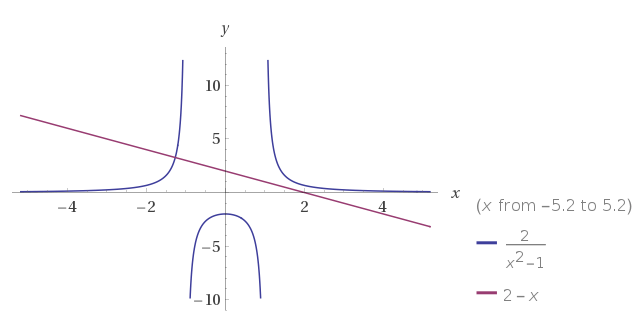
\includegraphics[width=14cm]{rozrahunkova_02/04_01.png}
  \label{fig:rr_02_04_01}
  \centering
\end{figure}

Судячи з графіку, задані лінії мають лише 1 точку пересічення $(\dfrac{2}{x^2-1} = 2-x)$, тому будемо вважати що таку площу знайти неможливо, оскільки вона нічим не обмежена.
 \\ \qquad \\
  % {\task{green}{В4 - РР1 - 04.02}} {\descr{Дослідити функцію на неперервність}}

$$
y=3^{\dfrac{2x}{3x+1}}
$$

Дослідимо функцію в точкі $-\dfrac{1}{3}$ де вона можливо має точку розриву.


$$
  \lim_{x \to -1/3 -0} 3^{\dfrac{2x}{3x+1}} \qquad \lim_{x \to (-1/3-0.001) -0} 3^{\dfrac{2x}{3x+1}} = \infty
$$

$$
  \lim_{x \to -1/3 +0} 3^{\dfrac{2x}{3x+1}} \qquad \lim_{x \to (-1/3+0.001) +0} 3^{\dfrac{2x}{3x+1}} = \infty
$$

\textbf{Висновок} - функція в точкі $-\dfrac{1}{3}$ тосить характер розриву \textbf{другого роду}, оскільки границі функції зліва та зправа прямують у нескінченність.


\begin{figure}[h!]
  \centering
  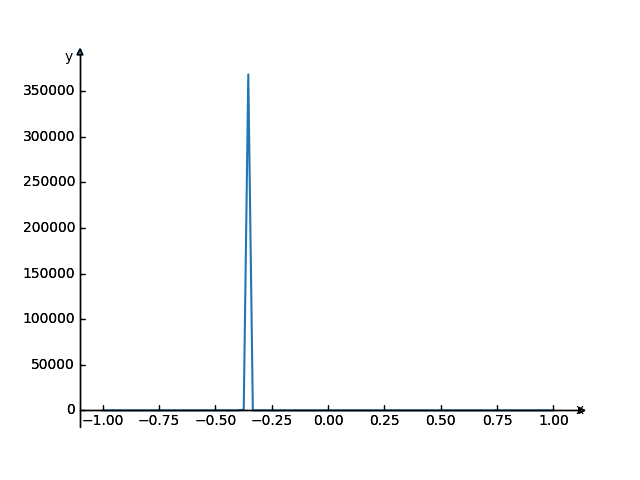
\includegraphics[width=14cm]{rozrahunkova_01/04_02.png}
  \caption{Графік функції}
  \label{fig:rr_01_40_02}
  \centering
\end{figure}
 \\ \qquad \\
  % {\task{green}{В4 - РР1 - 05.01}} {\descr[1]{Обчислити площу поверхні, одержаної при обертанні даннної кривої насколо осі OX}}

$$
  y = -\dfrac{1}{2}\ln{x}+\dfrac{x^2}{4} {\qquad} x \in [1;e]
$$

Для знаходження поверхні обертання використаємо наступну формулу

$$Q = 2\pi\int^b_a f(x) \sqrt{1+(f'(x))^2} \d{x} $$

$$
  2\pi \int^e_1 (-\dfrac{1}{2}\ln{x}+\dfrac{x^2}{4}) \sqrt{1+((\dfrac{x^2}{4}-\dfrac{1}{2}\ln{x})')^2} \d{x}
= 2\pi \int^e_1 \dfrac{1}{2} ( \dfrac{x^2}{2} - \ln{x} ) \sqrt{1+(\dfrac{x^2-1}{2x})^2} \d{x}
$$

$$
= \dfrac{2\pi}{2} ( \int^e_1  ( \dfrac{x^2}{2} - \ln{x} ) \sqrt{1+(\dfrac{x^2-1}{2x})^2} \d{x} )
= \pi \int^e_1  \dfrac{x^2}{2} \sqrt{1+(\dfrac{x^2-1}{2x})^2} \d{x} - \pi \int^e_1 \ln{x} \sqrt{1+(\dfrac{x^2-1}{2x})^2}
$$

$$
= \dfrac{\pi}{2} \int^e_1  x^2 \sqrt{\dfrac{4x^2+x^4-2x^2+1}{4x^2}} \d{x} - \pi \int^e_1 \ln{x} \sqrt{\dfrac{4x^2+x^4-2x^2+1}{4x^2}}\d{x}
$$

$$
= \dfrac{\pi}{2} \int^e_1  \dfrac{x^2}{2x} \sqrt{x^4+2x^2+1} \d{x} - \pi \int^e_1 \ln{x} \sqrt{\dfrac{x^2(x^2+2+\dfrac{1}{x^2})}{4x^2}}\d{x}
$$

$$
= \dfrac{\pi}{4} \int^e_1  x  \sqrt{(x^2+1)^2} \d{x} - \pi  \int^e_1 \dfrac{\ln{x}}{2} \sqrt{\dfrac{x^4+2x^2+1}{x^2}}\d{x}
$$

$$
= \dfrac{\pi}{4} \int^e_1  (x^3+x) \d{x} - \dfrac{\pi}{2}  \int^e_1 \ln{x} \sqrt{\dfrac{(x^2+1)^2}{x^2}}\d{x}
$$

$$
= \dfrac{\pi}{4} \int^e_1 x^3\d{x} + \dfrac{\pi}{4} \int^e_1 x \d{x} - \dfrac{\pi}{2}  \int^e_1  \dfrac{(x^2+1)\ln{x}}{x} \d{x}
$$

$$
= \dfrac{\pi}{4} \int^e_1 x^3\d{x} + \dfrac{\pi}{4} \int^e_1 x \d{x} - \dfrac{\pi}{2}( \int^e_1  \dfrac{x^2 \ln{x}}{x} \d{x} + \int^e_1 \dfrac{\ln{x}}{x} \d{x} )
$$


$$
= \dfrac{\pi}{4} \int^e_1 x^3\d{x} + \dfrac{\pi}{4} \int^e_1 x \d{x} - \dfrac{\pi}{2}\Bigg( \int^e_1  x\ln{x} \d{x} + \int^e_1 \dfrac{\ln{x}}{x} \d{x}
  \Bigg|
    \begin{array}{rlrlrlrl}
      u = & \ln{x} & x_1 = & e & y_1 = \ln{e} & = 1 \\
      u'= & \dfrac{1}{x} & x_0 = & 1 & y_0 = \ln{1} & = 0\\
      \end{array}
  \Bigg|
\Bigg)
$$

$$
= \dfrac{\pi}{4} \int^e_1 x^3\d{x} + \dfrac{\pi}{4} \int^e_1 x \d{x} - \dfrac{\pi}{2}( \int^e_1  x\ln{x} \d{x} + \int^1_0 u \d{u} )
$$

$$
= \dfrac{\pi}{4} \int^e_1 x^3\d{x} + \dfrac{\pi}{4} \int^e_1 x \d{x} - \dfrac{\pi}{2} \int^1_0 u \d{u}
 -  \dfrac{\pi}{2}\int^e_1  x\ln{x}  \d{x} \Bigg|
  \begin{array}{rlrl}
      u  =& \ln{x} & v  = & x^2/2 \\
      u' =& 1/x    & v' = & x \\
    \end{array}
\Bigg|
$$

$$
= \dfrac{\pi}{4} \int^e_1 x^3\d{x} + \dfrac{\pi}{4} \int^e_1 x \d{x} - \dfrac{\pi}{2} \int^1_0 u \d{u} -  \dfrac{\pi}{2} (\dfrac{x^2\ln{x}}{2} \Bigg|^e_1 - \int^e_1 \dfrac{1}{x} \dfrac{x^2}{2} \d{x} )
$$

$$
= \dfrac{\pi}{4} \int^e_1 x^3\d{x} + \dfrac{\pi}{4} \int^e_1 x \d{x} - \dfrac{\pi}{2} \int^1_0 u \d{u} -  \dfrac{\pi}{2} (\dfrac{x^2\ln{x}}{2} \Bigg|^e_1 - \dfrac{1}{2}\int^e_1 x\d{x} )
$$

Для більшої зручності порведемо обчислення визначених інтегралів окремо (формула вже завелика для копіювання навіть при наборі в LaTeX).

$$
1) \dfrac{\pi}{4} \int^e_1 x^3\d{x}
  = \dfrac{\pi}{4} \times \dfrac{x^4}{4}  \Bigg|^e_1
  = \dfrac{\pi}{16} (x^4) \Bigg|^e_1
  = \dfrac{\pi}{16} (e^4- 1^4)
  = \dfrac{\pi}{16} (e^4- 1)
$$

$$
2) \dfrac{\pi}{4} \int^e_1 x \d{x}
= \dfrac{\pi}{4} \times \dfrac{x^2}{2}  \Bigg|^e_1
= \dfrac{\pi}{8} (x^2) \Bigg|^e_1
= \dfrac{\pi}{8} (e^2 - 1^2)
= \dfrac{\pi}{8} (e^2 - 1)
$$


$$
3) - \dfrac{\pi}{2} \int^1_0 u \d{u} = - \dfrac{\pi}{4} (u^2)\Bigg|^1_0 = - \dfrac{\pi}{4} (1^2-0^2) = -\dfrac{\pi}{4}
$$

$$
4)  -  \dfrac{\pi}{2} \times \dfrac{x^2\ln{x}}{2} \Bigg|^e_1
= - \dfrac{\pi}{4} (e^2\ln{e}-1^2\ln{1})
= - \dfrac{\pi}{4} (e^2 \times 1 - 1^2 \times 0}) =
= - \dfrac{\pi e^2}{4}
$$

$$
5) - \dfrac{\pi}{2} \times -\dfrac{1}{2} \int^e_1 x\d{x}
= \dfrac{\pi}{4} \times \dfrac{x^2}{2}  \Bigg|^e_1
= \dfrac{\pi}{8} \times ( x^2 ) \Bigg|^e_1
= \dfrac{\pi}{8} \times ( e^2 - 1^2)
= \dfrac{\pi}{8} \times ( e^2 - 1)
$$

Залишилось лише просумувати отримані площі.

$$
\dfrac{\pi}{16} (e^4- 1) + \dfrac{\pi}{8} (e^2 - 1) -\dfrac{\pi}{4} - \dfrac{\pi e^2}{4} + \dfrac{\pi}{8} \times ( e^2 - 1)
= \dfrac{\pi}{16} (e^4- 1) + \dfrac{\pi}{4} (e^2 - 1) -\dfrac{\pi}{4} - \dfrac{\pi e^2}{4}
$$

$$
= \dfrac{\pi( (e^4-1) + 4(e^2-1) - 4 -4e^2)}{16}
= \dfrac{\pi( e^4-1 + 4e^2-4 - 4 -4e^2)}{16}
= \dfrac{\pi( e^4-9 ) }{16}
$$


$$
\boxed{ Q = \dfrac{\pi( e^4-9 ) }{16} }
$$
 \\ \qquad \\
  % {\task{green}{В4 - РР1 - 05.02}} {\descr{Знайти похідну функції:}}

$$
  y = \sqrt{x^3+2x+\dfrac{1}{x}} = (x^3+2x+\dfrac{1}{x})^{\dfrac{1}{2}}
$$

$$
  y' = ((x^3+2x+\dfrac{1}{x})^{\dfrac{1}{2}})'
     =  \dfrac{1}{2}(x^3+2x+\dfrac{1}{x})^{-\dfrac{1}{2}}(x^3+2x+\dfrac{1}{x})'
     =  \dfrac{1}{2}(x^3+2x+\dfrac{1}{x})^{-\dfrac{1}{2}}(3x^2+2+\dfrac{1}{x^2})
$$

$$
  y' = \dfrac{3x^2+2+\dfrac{1}{x^2}}{2\sqrt(x^3+2x+\dfrac{1}{x})}
$$
 \\ \qquad \\
  % {\task{green}{В4 - РР1 - 05.03}} {\descr{Знайти похідну функції:}}

$$
  y = \dfrac{\arccos\sqrt{x}}{x}
$$
$$
  y' = \dfrac{(\arccos\sqrt{x})'(x)-(\arccos\sqrt{x})(x)'}{x^2}
     = \dfrac{-\dfrac{x}{\sqrt{1-(\sqrt{x})^2}}(\sqrt{x})'-\arccos\sqrt{x}}{x^2} =
$$
$$
    = \dfrac{-\dfrac{x}{\sqrt{1-x}}\cdot\dfrac{1}{2\sqrt(x)}-\arccos\sqrt{x}}{x^2}
     = - \dfrac{\dfrac{x}{2\sqrt{x}\sqrt{1-x}}+\arccos\sqrt{x}}{x^2}.
$$
 \\ \qquad \\
  % {\task{green}{В4 - РР1 - 05.04}} {\descr{Знайти похідну функції:}}

$$
  \begin{array}{r c l}
    y  & = & (x^3-x^2)^x \\
    y' & = & ((x^3-x^2)^x)' \\
    (\ln y)' & = & (\ln(x^3-x^2)^x)' \\
    \\
    \dfrac{1}{y}y' & = & x \dfrac{1}{x^3-x^2}(x^3-x^2)' \\
  \end{array}
$$

$$
  y' = x(x^3-x^2)^x \dfrac{1}{x^3-x^2}(3x^2-2x)
      = \dfrac{x (x^3-x^2)^x(3x^2-2x)}{x^3-x^2}
$$
$$
  y' = (x^3-x^2)^{x-1}(3x^3-2x^2).
$$

% \begin{array}{r c l}
%   \dfrac{1}{y}y' & = & x \dfrac{1}{x^3-x^2}(x^3-x^2)' \\
%   \dfrac{y'}{y}  & = & x \dfrac{1}{x^3-x^2}(3x^2-2x) \\
%   y' & = & x (x^3-x^2)^x \dfrac{1}{x^3-x^2}(3x^2-2x) \\
%   y' & = & \dfrac{x (x^3-x^2)^x(3x^2-2x)}{x^3-x^2} \\
%   \\
%   y' & = & \dfrac{(x^3-x^2)^x(3x^3-2x^2)}{x^3-x^2} \\
%   \\
%   y' & = & (3x^3-2x^2)(x^3-x^2)^{x-1} \\
%   \end{array}
 \\ \qquad \\
  % {\task{green}{В4 - РР1 - 05.05}} {\descr{Знайти похідну функції:}}

$$
 y = 5^{\tg^2{x}}
$$

$$
y' = (5^{\tg^2{x}})' = 5^{\tg^2{x}} \cdot \ln{5} \cdot ((\tg{x})^2)' = 5^{\tg^2{x}} \cdot \ln{5} \cdot 2 \tg{x} \cdot \dfrac{1}{\cos^2{x}}
$$
 \\ \qquad \\
  % {\task{green}{В4 - РР1 - 05.06}} {\descr{Знайти похідну функції:}}

$$
x\tg{y}-y{\tg{x}} = 2
$$

$$
x\tg{y}-y{\tg{x}} - 2 = 0
$$

$$
 0 = (x\tg{y})'-(y{\tg{x}})' - (2)' = ( (x)'\tg{y} + x(\tg{y})' ) - ((y)'\tg{x} + y(\tg{x})') = (x'\tg{y} + \dfrac{x}{\cos^2{y}}) - (y'\tg{x}+\dfrac{y}{\cos^2{x}})
$$

$$
y'\tg{x}+\dfrac{y}{\cos^2{x}} = x'\tg{y} + \dfrac{x}{\cos^2{y}}
$$

$$
y'\tg{x}
  = x'\tg{y} + \dfrac{x}{\cos^2{y}} - \dfrac{y}{\cos^2{x}}
$$

$$
  y' = \dfrac{\tg{y}}{\tg{x}}   + \dfrac{x}{\tg{x}\cos^2{y}}   - \dfrac{y}{\tg{x}\cos^2{x}}
$$
 \\ \qquad \\
  % {\task{green}{В4 - РР1 - 05.07}} {\descr{Знайти похідну функції:}}

\begin{displaymath}
  \left\{\begin{array}{rl}
    x =& \dfrac{1}{t+2} \\
    y =& \dfrac{t^2}{(t+2)^2}
  \end{array} \qquad y'_x=? \qquad y''_xx=?
\end{displaymath}

$$
  y'_x=\dfrac{y'}{x'} \qquad y''_xx=\dfrac{y'_x}{x'}
$$

$$
  x' = \Big(\dfrac{1}{t+2}\Big)' = \dfrac{1}{(t+2)^2}(t+2)' = \dfrac{1}{(t+2)^2}
$$

$$
  y' = \Big(\dfrac{t^2}{(t+2)^2}\Big)'
     = \dfrac{(t^2)'(t+2)^2-(t^2)((t+2)^2)'}{(t+2)^4}
     = \dfrac{2t(t+2)^2-2t^2(t+2)}{(t+2)^4}
     = \dfrac{(2t(t+2)-2t^2)(t+2)}{(t+2)^4}
$$
$$
  y' = \dfrac{2t(t+2)-2t^2}{(t+2)^3} = \dfrac{2t((t+2)-t)}{(t+2)^3}= \dfrac{4t}{(t+2)^3}
$$

$$
  y'_{x}
    = \dfrac{y'}{x'}
    = \dfrac{\dfrac{4t}{(t+2)^3}}{\dfrac{1}{(t+2)^2}}
    = \dfrac{4t(t+2)^2}{(t+2)^3}
    = \dfrac{4t}{t+2}
$$

$$
  y''_{xx} = \dfrac{(y'_{x})'}{x'}
    = \dfrac{\Big(\dfrac{4t}{t+2}\Big)'}{\dfrac{1}{(t+2)^2}}
    = (t+2)^2 \dfrac{(4t)'(t+2)-(4t)(t+2)'}{(t+2)^2}
    = \dfrac{(4t+8-4t)(t+2)^2}{(t+2)^2} = 8
$$
 \\ \qquad \\
  %
  % {\task{green}{В4 - РР1 - 06.01}} {\descr[1]{Знайти обєм тіла, одержаного прі обертанні криволінійного заданого сектора навколо полярної осі:}}

$$
\rho = \alpha \sqrt{\cos{\varphi}},{\qquad} \varphi \in \Big[ 0; \dfrac{\pi}{2} \Big]
$$

Об'єм  тіла  отирманого обертанням в навколо полярної осі заданого двума поялрними координатами можна знайти за формулою
$$
V = \dfrac{2\pi}{3} \int_{\alpha}^{\beta} \rho^3\sin{\varphi} \d{\varphi}
$$

% http://energy.bmstu.ru/gormath/mathan2s/usint/UsingInt.htm#s121
$$
\dfrac{2\pi}{3} \int_0^{\dfrac{\pi}{2}} (a\sqrt{\cos{\varphi}})^3\sin{\varphi} \d{\varphi}
= \dfrac{2\pi}{3} \int_0^{\dfrac{\pi}{2}} a^3 \cos{\varphi}^{\dfrac{3}{2}}  \sin{\varphi} \d{\varphi}
\Bigg|
  \begin{array}{rl rl r}
     u =& \sin{\varphi} & \varphi_2 = & \dfrac{\pi}{2} & u_2 =   1  \\
    \d{u} =& \cos{\varphi} & \varphi_1 = & 0 & u_1 =   0 \\
  \end{array}
\Bigg| = \dfrac{2\pi a^4 }{3} \int^1_0 u^{\dfrac{3}{2}}\d{u}
$$

$$
= \dfrac{2\pi a^4 }{3} \int^1_0 u^{\dfrac{3}{2}}\d{u}
= \dfrac{a^4 \pi}{6} \dfrac{u^{\dfrac{5}{2}}}{\dfrac{5}{2}} \Bigg|_0^{1}
= \dfrac{a^4 \pi}{15} \sqrt{u^5} \Bigg|_0^{1}
= \dfrac{a^4 \pi}{15}
$$

$$
\boxed{V = \dfrac{a^4 \pi}{15} }
$$
 \\ \qquad \\
  % {\task{green}{В4 - РР1 - 07.01}} {\descr{Провести повне дослідження функції і побудувати графік}}

$$
y=\dfrac{2}{x^2+2x}
$$


1) $x \in (-\infty;-2)\cup(-2;0)\cup(0;+\infty)$

2) Графік не перетинає ось $x$.

3) Функція непарна оскільки

$$
  f(-x) = \dfrac{2}{(-x)^2+2(-x)} = \dfrac{2}{x^2-2x}
$$

4) Обидві точки -2 та 0 носить характер розриву другого роду оскільки вони прямують в безмежність.

$$
  \lim_{x \to -2 \ \pm0} \dfrac{2}{x^2+2x} = \mp \infty \qquad   \lim_{x \to 0 \ \pm0} \dfrac{2}{x^2+2x} = \pm \infty
$$

5) Похідна
$$
  y' = (\dfrac{2}{x^2+2x})'
     = \dfrac{2'(x^2+2x)-2(x^2+2x)'}{(x^2+2x)^2}
     = \dfrac{-4x-4}{(x^2+2x)^2}
$$

Функція не існує в точках $x=-2$ та $x=0$, а $x=-1$ є критичною (такою що є підозрілою на екстремум мінімум або максимум). На інтервалі $(-\infty;+\infty)$ матимемо:



\begin{center}
  \begin{tabular}{ | c | c | c | c | c | c | c | c | }
    \hline
      x     & (-\infty;-2) & -2 & (-2;-1) & -1 & (-1:0) & 0 &  (0; +\infty) \\
      \hline
      f'(x) &  + & не існує & + & 0  & -  & не існує & - \\
      \hline
      f(x)  & \nearrow  & не існує & \nearrow  & y_{max} = -2  & \searrow   & не існує & \searrow \\
    \hline
  \end{tabular}
\end{center}



6) Друга похідна

$$
  y'' = (\dfrac{-4x-4}{(x^2+2x)^2})'
  = \dfrac{(-4x-4)'(x^2+2x)^2 - (-4x-4)((x^2+2x)^2)' }{(x^2+2x)^4}
$$

$$
= \dfrac{-4(x^2+2x) + 4(2x+2)^2 }{(x^2+2x)^3}
= \dfrac{-4x^2-8x + 16x^2+32x+16 }{(x^2+2x)^3}
= \dfrac{12x^2+24x+16 }{(x^2+2x)^3}
$$

\begin{center}
  \begin{tabular}{ | c | c | c | c | c | c |  }
    \hline
    x & (-\infty;-2) & -2 & (-2:0) & 0 & (0:+\infty) \\
    \hline
    f"(x) &  + & не існує  & - & не існує & +  \\
    \hline
    f(x) &  \cup & не існує  & \cap & не існує & \cup \\
    \hline
  \end{tabular}
\end{center}

7) з пункта (4) випливає що фунція має вертикальні асимптоти в точках $x=-2$ та $x=0$.

Знаходимо горизонтальні асимптоти за формулами (через границі функції):
$$
  y = kx+b
$$

$$
  k = \lim_{x\to\infty} \dfrac{y(x)}{x}
    = \lim_{x\to\infty} \dfrac{2}{x(x^2+2x)}
    = \lim_{x\to\infty} \dfrac{2/x^2}{x(1+2/x)}
    = \dfrac{1}{\infty}
    = 0
$$

$$
  b = \lim_{x\to\infty} (y(x) - kx)
    = \lim_{x\to\infty} \dfrac{2}{x^2+2x}
    = \lim_{x\to\infty} \dfrac{2/x^2}{1+2/x}
    = \dfrac{0}{1}
    = 0
$$

8) Враховуючи висновки ослідження функції будуємо графік:

\begin{figure}[h!]
  \centering
  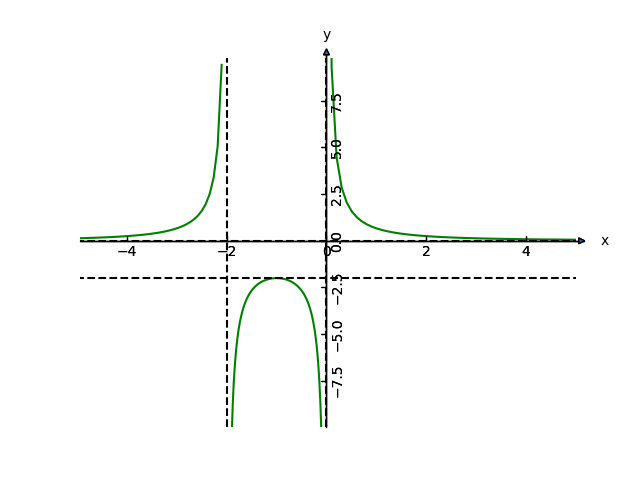
\includegraphics[width=14cm]{rozrahunkova_01/07_01.png}
  \caption{Графік функції $y=\dfrac{2}{x^2+2x}$ }
  \label{fig:rr_01_07_01}
  \centering
\end{figure}
 \\ \qquad \\
  % {\task{gray}{В4 - РР1 - 07.02}} {\descr{Провести повне дослідження функції і побудувати графік}}

$$
\rho =\alpha (1-cos2\varphi)
$$
 \\ \qquad \\

  % % інтеграли
  % {\task{green}{В4 - РР2 - 01.01}} \begin{center}\large{\cyr{\textbf{1.1 Довести тотожність аксіоматично}}}\end{center}

\begin{displaymath}
  A\cup((B\bigtriangleup(B\bigtriangleup{A})) \setminus B)=A
\end{displaymath}

Спростимо ліву частину завдиння поступово спрощуючи формули за допомогою основних та похідних законів алгебри множин (для кращого розуміння ходу процесу кожна дія обмежена одною-двома операціями):

$$
A\cup((B\bigtriangleup(B\bigtriangleup{A})) \setminus B) = A
$$

\begin{displaymath}


  \text{ Операції $\setminus$ та $\bigtriangleup$ розкривати за формулами: }\\
  A\setminus{B}=A\cap{B}\compl \\qquad A\bigtriangleup{B} = (A\cap{B\compl})\cup{(B\cap{A\compl} )}

\end{displaymath}

\begin{center}\normalsize{\cyr{\textbf{Розкриття}}}\end{center}
\begin{array}{l}

  A = A\cup{((B\bigtriangleup(B\bigtriangleup{A})) \setminus B)}   \\
  A = A\cup{((B\bigtriangleup(  ( ( A\compl \cap{B} )  \cup{ ( A \cap{B\compl} )} )  )) \setminus B)}   \\
  A = A\cup{(( (  ( ( A\compl \cap{B} )  \cup{ ( A \cap{B\compl} )} ) \compl \cap{B} )  \cup{ (  ( ( A\compl \cap{B} )  \cup{ ( A \cap{B\compl} )} )  \cap{B\compl} )} )  \setminus B)}  \\

  A = A\cup{((((( A\compl \cap{B} )  \cup{ ( A \cap{B\compl} )} ) \compl \cap{B} )  \cup{ (  ( ( A\compl \cap{B} )  \cup{ ( A \cap{B\compl} )} )  \cap{B\compl} )} )  \cap{B\compl} )}   \\

\end{array}


\begin{center}\normalsize{\cyr{\textbf{Доведення}}}\end{center}
$$
\begin{array}{r|l}
  \text{Закони} & \text{Тотожності} \\
  \hline \\
  1      & A \cup ( B\compl \cap ( ( B \cap ( ( A\compl \cap{B}) \cup ( A \cap B\compl ) )\compl ) \cup ( {B\compl} \cap ( ( A\compl\cap{B}) \cup (A \cap B\compl)) )) ) \\
  10,11,1  & A \cup ( B\compl \cap ( ( B \cap  ( ( A\compl \cup B ) \cap ( A \cup B\compl ) ) ) \cup ( B\compl \cap ( ( A\compl \cap B ) \cup ( A \cap B\compl ) ) ) ) ) \\
  2      & A \cup ( B\compl \cap ( ( ( B \cap ( A\compl \cup  B ) ) \cap ( B \cap (  A \cup B\compl ) ) ) \cup ( (B\compl \cap ( A\compl \cap  B ) ) \cap ( B\compl \cap ( A \cap B\compl ) ) ) ) ) \\
  1       & A \cup ( B\compl \cap ( ( ( B \cap (  B \cup A\compl ) ) \cap ( B \cap ( B\compl \cup  A ) ) ) \cup ( (B\compl \cap (  B \cap A\compl ) ) \cap ( B\compl \cap ( B\compl \cap A ) ) ) ) ) \\
  6       & A \cup ( B\compl \cap ( ( ( B \cap ( B \cup A\compl ) ) \cap ( B \cap ( B\compl \cup  A ) ) ) \cup ( (B\compl \cap (  B \cap A\compl ) ) \cap ( B\compl \cap ( B\compl \cap A ) ) ) ) ) \\
  12      & A \cup ( B\compl \cap ( ( B \cap ( B \cap ( B\compl \cup  A ) ) ) \cup ( (B\compl \cap (  B \cap A\compl ) ) \cap ( B\compl \cap ( B\compl \cap A ) ) ) ) ) \\
  8       & A \cup ( B\compl \cap ( ( ( B \cap B )  \cap A  ) \cup ( ( ( B\compl \cap B )  \cap A\compl ) \cap ( ( B\compl \cap B\compl ) \cap A  ) ) ) ) \\
  5,4,7   & A \cup ( B\compl \cap ( ( B \cap A ) \cup ( ( \emptyset \cap A\compl ) \cap (B\compl \cap A ) ) ) \\
  5       & A \cup ( B\compl \cap ( ( B \cap A ) \cup ( \emptyset \cap (B\compl \cap A ) ) ) \\
  3       & A \cup ( B\compl \cap ( ( B \cap A ) \cup \emptyset   ) \\
  8,4       & A \cup ( B\compl \cap ( B \cap A ) ) \\
  5       & A \cup ( \emptyset \cap A   ) \\
  5       & A \cup \emptyset  \\
  3       & A

\end{array}
$$

Тотожність доведено.
 \\ \qquad \\
  % {\task{green}{В4 - РР2 - 01.02}} {\descr{Знайти Інтеграл}}

$$
\int \dfrac{\d{x}}{1+cos2x} = \Bigg |
  \begin{array}{r l }
    \cos^2x = & \dfrac{1+cos2x}{2} \\
    2 \cos^2x = & 1+cos2x \\
  \end{array}
\Bigg |
$$

$$
  \int \dfrac{\d{x}}{2\cos^2x}
  = \dfrac{1}{2} \int \dfrac{\d{x}}{\cos^2x}
  = \dfrac{1}{2} \cdot \tg{x} + C
  = \frac{tg{x}}{2} + C.
$$

$$
  \boxed{\frac{tg{x}}{2} + C}
$$
 \\ \qquad \\
  % {\task{green}{В4 - РР2 - 01.03}} {\descr{Знайти Інтеграл}}

$$
  \int \dfrac{2x\d{x}}{x^4+3}
= \int 2x \dfrac{1}{x^4+3} \d{x}
= \Bigg|
    \begin{array}{c l}
      t = x^2   & \d{x} = (x)'dt \\
      x = \sqrt{t} & \d{x} = \dfrac{1}{2\sqrt{t}}\d{t}
      \end{array}
  \Bigg|
$$

$$
  2 \int \dfrac{\sqrt{t}}{2(t^2+3)(\sqrt{t})}\d{t}
= \dfrac{2}{2} \int \dfrac{\sqrt{t}}{(t^2+3)(\sqrt{t})}\d{t}
= \int \dfrac{1}{t^2+\sqrt{3}^2}\d{t}
= \dfrac{arctg{\dfrac{t}{\sqrt{3}}}}{\sqrt{3}} + C
= \dfrac{arctg{\dfrac{x^2}{\sqrt{3}}}}{\sqrt{3}} + C.
$$


$$
  \boxed{\dfrac{arctg{\dfrac{x^2}{\sqrt{3}}}}{\sqrt{3}} + C}
$$
 \\ \qquad \\
  % {\task{green}{В4 - РР2 - 01.04}} {\descr{Знайти Інтеграл}}


$$
  \int \dfrac{\d{x}}{\sqrt{3-2x}} =
    \Bigg |
      \begin{array}{l c  l}
        t = 3-2x & & \d{x} = (x)'\d{t}  \\
        x = \dfrac{3-t}{2} & & \d{x} = (\dfrac{3}{2} - \dfrac{t}{2})' = \dfrac{\d{t}}{2} \\
      \end{array}
    \Bigg |
$$

$$
\int \dfrac{1}{2} \cdot \dfrac{\d{t}}{\sqrt{t}} =
\dfrac{1}{2} \int t^{-\dfrac{1}{2}}dt =
\dfrac{1}{2} \cdot \dfrac{t^{-\dfrac{1}{2}+1}}{\dfrac{1}{2}} + C =
\dfrac{1}{2} \cdot \dfrac{2}{1} \cdot \sqrt{t} + C = \sqrt{t} + C =
\Big |
  \begin{array}{c}
    t = 3-2x
  \end{array}
\Big | =
\sqrt{3-2x} + C.
$$

$$
\boxed{\sqrt{3-2x} + C}
$$
 \\ \qquad \\
  % {\task{green}{В4 - РР2 - 01.05}} {\descr{Знайти Інтеграл}}

$$
  \int \dfrac{\ln{\tg{x}}}{\sin{2x}}\d{x}
= \int \ln{\tg{x}} \dfrac{1}{2\sin{x}\cos{x}}\d{x}

$$

Якщо провести заміну $t = \ln{\tg{x}}$ і позначити $\d{t}$ як $t'\d{x}$ то можемо бачити що:

$$
\d{u}
= (\ln{\tg{x}})'\d{x} = \dfrac{1}{\tg{x}} \tg{x}' \d{x}
= \dfrac{1}{\dfrac{\sin{x}}{\cos{x}}} \cdot   \dfrac{1}{\cos^2{x}}  \d{x}
= \dfrac{1}{\sin{x}\cos{x}}  \d{x}
$$

Як бачимо цей вираз вже присутній під інтегралом, отож можемо провести заміну:

$$
  \dfrac{1}{2} \int t\d{t}
= \dfrac{1}{2} \cdot \dfrac{t^2}{2} + C
= \dfrac{t^2}{4} + C =
= \dfrac{(\ln{\tg{x}})^2}{4} + C.
$$

$$
\boxed{\dfrac{(\ln{\tg{x}})^2}{4} + C}
$$
 \\ \qquad \\
  % {\task{green}{В4 - РР2 - 01.06}} {\descr{Знайти Інтеграл}}


$$
  \int \dfrac{x\d{x}}{\sqrt{x^2+3x-1}}
= \int \dfrac{x\d{x}}{\sqrt{(x+\dfrac{3}{2})^2-\dfrac{13}{4}}}
= \Bigg |
  \begin{array}{rrrl}
    t = & x + \dfrac{3}{2} & \d{x} =& (x)'\d{t}\\
    \\
    x = & t - \dfrac{3}{2} & \d{x} =& \d{t}\\
  \end{array}
\Bigg |
= \int \dfrac{t-\dfrac{3}{2}}{\sqrt{t^2-\dfrac{13}{4}}} \d{t}
$$

$$
\int \dfrac{t\d{t}}{\sqrt{t^2-\dfrac{13}{4}}}  - \int \dfrac{\dfrac{3}{2}\d{t}}{\sqrt{t^2-\dfrac{13}{4}}}
= \int \dfrac{t\d{t}}{\sqrt{t^2-\dfrac{13}{4}}}  - \dfrac{3}{2} \int \dfrac{\d{t}}{\sqrt{t^2-\dfrac{13}{4}}}
=
$$

Окремо проінтегруємо обидва інтеграли:

$$
1)  \int \dfrac{t\d{t}}{\sqrt{t^2-\dfrac{13}{4}}}
= \int (t^2-\dfrac{13}{4})^{-\dfrac{1}{2}} \cdot t\d{t}
= \dfrac{2}{2} \int (t^2-\dfrac{13}{4})^{-\dfrac{1}{2}} \cdot t\d{t}
= \dfrac{1}{2} \int (t^2-\dfrac{13}{4})^{-\dfrac{1}{2}} \cdot 2t\d{t}
$$

$$
= \dfrac{1}{2} \int (t^2-\dfrac{13}{4})^{-\dfrac{1}{2}} \cdot \d{(t^2-\dfrac{13}{4})}
= \dfrac{2 \sqrt{t^2-\dfrac{13}{4}}}{2} + C
= \sqrt{(x + \dfrac{3}{2})^2-\dfrac{13}{4}} + C
= \sqrt{x^2+3x-1} + C.
$$


$$
2)
  - \dfrac{3}{2} \int \dfrac{\d{t}}{\sqrt{t^2-\dfrac{13}{4}}} = - \dfrac{3}{2}  ln \Bigg|t + \sqrt{t^2-\dfrac{13}{4}}\Bigg| + C = - \dfrac{3}{2}  ln \Bigg|x + \dfrac{3}{2} + \sqrt{(x + \dfrac{3}{2})^2-\dfrac{13}{4}}\Bigg| + C
$$

Підставимо обидва розвязки назад в нашу формулу і отримаємо рішення:

$$
\sqrt{x^2+3x-1} - \dfrac{3 \ln{\bigg|x + \dfrac{3}{2} + \sqrt{x^2+3x-1}\bigg|} }{2} + C
$$
 \\ \qquad \\
  % {\task{green}{В4 - РР2 - 01.07}} {\descr{Знайти Інтеграл}}

$$
  \int (x+5)\ln{x}\d{x} =
  \Bigg|
    \begin{array}{r l r l   }
        u  & = \ln{x} & v & = \dfrac{x^2}{2}+5x \\
        u' & = \dfrac{1}{x} & v' & = x+5  \\
      \end{array}
  \Bigg|
$$


$$
  \int (x+5)\ln{x}\d{x}
= \ln{x} (\dfrac{x^2}{2}+5x) - \int (\dfrac{x^2}{2}+5x) \dfrac{1}{x} \d{x}
$$
$$
= \ln{x} (\dfrac{x^2}{2}+5x) - \int \dfrac{x^2+10x}{2x}\d{x}
= \ln{x} (\dfrac{x^2}{2}+5x) - \dfrac{1}{2}\int \dfrac{x(x+10)}{x}\d{x}
$$

$$
= \ln{x} (\dfrac{x^2}{2}+5x) - \dfrac{1}{2} ( \int x\d{x} + \int 10\d{x} )
= \ln{x} (\dfrac{x^2}{2}+5x) - \dfrac{1}{2} ( \dfrac{x^2}{2} + 10x) + C
$$

$$
= \ln{x} (\dfrac{x^2}{2}+5x) - ( \dfrac{x^2}{4} + 5x) + C
= 5x\ln{x} + \dfrac{x^2}{2}\ln{x} - \dfrac{x^2}{4} - 5x + C
= 5x(\ln{x}-1) + \dfrac{1}{2}(\ln{x}-\dfrac{1}{2}) + C
$$

$$\boxed{5x(\ln{x}-1) + \dfrac{1}{2}(\ln{x}-\dfrac{1}{2}) + C}$$
 \\ \qquad \\
  % {\task{green}{В4 - РР2 - 01.08}} {\descr{Знайти Інтеграл}}

$$
  \int (x+1)2^x\d{x} =  \int x2^x\d{x} + \int 2^x\d{x} = \int x2^x\d{x} + \dfrac{2^x}{\ln{2}} + C
$$

$$
\int x2^x\d{x}
= \Bigg |
  \begin{array}{rlrl}
    u  &= x & v =& \dfrac{2^x}{\ln{2}} \\
    \\
    u' &= 1 & v'=& 2^x \\
  \end{array}
\Bigg |
= x \dfrac{2^x}{\ln{2}} - \int \dfrac{2^x}{\ln{2}}\d{x}
= \dfrac{x2^x}{\ln{2}} - \dfrac{1}{\ln{2}}\int  2^x\d{x}
= \dfrac{x2^x}{\ln{2}} - \dfrac{1}{\ln{2}} \cdot \dfrac{2^x}{\ln{2}} + C
$$


$$
  \int (x+1)2^x\d{x}  = \dfrac{x2^x}{\ln{2}} - \dfrac{2^x}{(\ln{2})^2} + \dfrac{2^x}{\ln{2}} + C = \dfrac{2^x}{\ln{2}} \Big( x - \dfrac{1}{\ln2}+1 \Big) + C
$$


$$\boxed{ \dfrac{2^x}{\ln{2}} \Big( x - \dfrac{1}{\ln2}+1 \Big) + C }$$
 \\ \qquad \\
  % {\task{green}{В4 - РР2 - 01.09}} {\descr{Знайти Інтеграл}}

$$
  \int \dfrac{2x^4-9x^2-1}{x^3-7x-6}\d{x} = \int \dfrac{2x^4-9x^2-1}{(x+1)(x+2)(x-3)}\d{x}
$$

Розкладаємо многочлен:

\begin{center}
  \begin{tabular}{r r | l}
      & 2x^4-9x^2+0x-1   & x^3-7x-6 \\ \cline{3-1}
    - & 2x^4-14x^2-12x+0 & 2x       \\ \cline{2-1}
      &   5x^2+12x-1 & \\

  \end{tabular}
\end{center}

В свою чергу розкладаємо многочлен що залишився:

$$
  \dfrac{5x^2+12x-1}{(x+1)(x+2)(x-3)}
    = \dfrac{A}{x+1} + \dfrac{B}{x+2} + \dfrac{C}{x-3}
    = \dfrac{A(x+2)(x-3)+B(x+1)(x-3)+C(x+1)(x+2)}{(x+1)(x+2)(x-3)}
$$

$$
5x^2+12x-1 = A(x^2-3x+2x-6)+B(x^2-3x+x-3)+C(x^2+2x+1x+2)
$$


$$
  \begin{array}{r|c|r}
    x^2 & 5  & A+B+C      \\
    x^1 & 12  & -A-2B+3B  \\
    x^0 & -1  & -6A-3B+2C \\
    \end{array}
    \hspace{2pt}
    {\text{з чого виходить що}}
    \hspace{2pt}
    A=2, B=-1, C=4
$$

З чого (після підстановки) отримуємо спрощений інтеграл:

$$
   \int 2x + \dfrac{2}{x+1} - \dfrac{1}{x+2} + \dfrac{4}{x-3}  \d{x}
= 2\int x \d{x} + 2 \int \dfrac{\d{x}}{x+1} - \int \dfrac{\d{x}}{x+2} + 4 \int \dfrac{\d{x}}{x-3}
$$

$$
\boxed{x^2 + 2 \ln{|x+1|} - \ln{|x+2|} + 4\ln{|x-3|} + C}.
$$
 \\ \qquad \\
  % {\task{green}{В4 - РР2 - 01.10}} {\descr{Знайти Інтеграл}}
$$
  \int \dfrac{4x^4+8x^3-1}{(x^2-1)(x+1)}\d{x}
= \int \dfrac{4x^4+8x^3-1}{(x-1)(x+1)(x+1)}\d{x}
= \int \dfrac{4x^4+8x^3-1}{x^3+x^2-x^1-1}\d{x}
$$

Розкладаємо многочлен:

\begin{center}
  \begin{tabular}{r r | l}
      & 4x^4+8x^3+0x^2+0x-1 & x^3+x^2-x^1-1 \\ \cline{3-1}
    - & 4x^4+4x^3-4x^2-4x-0 & 4x + 4        \\ \cline{2-1}
      & 4x^3+4x^2+4x-1  & \\
    - & 4x^3+4x^2-4x-4  & \\   \cline{2-1}
      & 8x+3  & \\
  \end{tabular}
\end{center}

В свою чергу розкладаємо многочлен що залишився:

$$
  \dfrac{8x+3}{(x-1)(x+1)(x+1)}
    = \dfrac{A}{x-1} + \dfrac{B}{x+1} + \dfrac{C}{(x+1)^2}
    = \dfrac{A(x+1)^2+B(x-1)(x+1)+C(x-1)}{(x-1)(x+1)(x+1)}
$$

$$
   8x+3 = A(x^2+2x+1)+B(x^2-1)+C(x-1)
$$

$$
  \begin{array}{r|c|r}
    x^2 & 0  & A+B   \\
    x^1 & 8  & 2A-C  \\
    x^0 & 3  & A-B-C \\
    \end{array}
    \hspace{2pt}
    {\text{з чого виходить що}}
    \hspace{2pt}
    A=\dfrac{11}{4}, B=-\dfrac{11}{4}, C=\dfrac{5}{2}
$$

З чого (після підстановки) отримуємо спрощений інтеграл:

$$
  \int 4x+4+ \dfrac{\dfrac{11}{4}}{x-1}+\dfrac{-\dfrac{11}{4}}{x+1}+\dfrac{\dfrac{5}{2}}{(x+1)^2} \d{x} = \int 4x+4+ \dfrac{11}{4(x-1)}-\dfrac{11}{4(x+1)}+\dfrac{5}{2(x+1)^2} \d{x} =
$$

$$
4\int x\d{x} + 4\int\d{x}+ \dfrac{11}{4}\int\dfrac{\d{x}}{(x-1)}-\dfrac{11}{4}\int\dfrac{\d{x}}{(x+1)}+\dfrac{5}{2}\int\dfrac{\d{x+1}}{(x+1)^2} =
$$

$$
\boxed{2x^2+4x+\dfrac{11}{4}(\ln{|x-1|}-\ln{|x+1|})+\dfrac{5}{2(x+1)}+C}
$$
 \\ \qquad \\
  % {\task{green}{В4 - РР2 - 01.11}} {\descr{Знайти Інтеграл}}

$$
  \int \dfrac{(x^2+23)\d{x}}{(x+1)(x^2+6x+13)}
$$

Спершу, cпрощуємо многочлен:
$$
  \dfrac{(x^2+23)\d{x}}{(x+1)(x^2+6x+13)}
= \dfrac{A}{(x+1)} + \dfrac{Bx+C}{(x^2+6x+13)}
= \dfrac{A(x^2+6x+13) + (Bx+C)(x+1)}{(x+1)(x^2+6x+13)}
$$
$$
  (x^2+23) = A(x^2+6x+13) + (Bx+C)(x+1) = Ax^2+6Ax+13A+Bx^2+Bx+Cx+C
$$

$$
  \begin{array}{rcl}
    x^2 & 0  & A+B\\
    x^1 & 1  & 6A+B+C\\
    x^0 & 23 & 13A+C
    \end{array}
    \hspace{2pt}
    {\text{з чого виходить що}}
    \hspace{2pt}
    A=3, B=-2, C=-16
$$

$$
  \int \dfrac{3}{x+1}\d{x} + \int \dfrac{-1(2x+16)}{x^2+6x+13}
= 3\int \dfrac{1}{x+1}\d{x} - \int \dfrac{2x+16}{x^2+6x+13}\d{x}
$$

$$
= 3\int \dfrac{1}{x+1}\d{x} - \int \dfrac{2x+6}{x^2+6x+13}\d{x} - \int \dfrac{10}{x^2+6x+13}\d{x}
$$

$$
= 3 \ln{|x+1|} + C - \int \dfrac{\d{x^2+6x+13}}{x^2+6x+13} - 10\int \dfrac{1}{x^2+6x+13}\d{x}
$$

$$
= 3 \ln{|x+1|} - \ln{|x^2+6x+13|} + C + 10\int \dfrac{1}{(x+3)^2+4}\d{x}
\Bigg|
  \begin{array}{rlrl}
    t = & x+3   & \d{x} = & (x)'\d{t}\\
    x = & t - 3 & \d{x} = & \d{t} \\
    \end{array}
\Bigg| =
$$

$$
  = 3 \ln{|x+1|} - \ln{|x^2+6x+13|} + C - 10\int \dfrac{1}{t^2+4}\d{t}
$$

$$
= 3 \ln{|x+1|} - \ln{|x^2+6x+13|} + C - \dfrac{10}{4}\int \dfrac{1}{\dfrac{t^2}{4}+1}\d{t}
\Bigg|
  \begin{array}{rlrl}
    u = & \dfrac{t}{2}   & \d{t} = & (t)'\d{u}\\
    t = & 2u & \d{t} = & 2\d{u} \\
    \end{array}
\Bigg|
$$

$$
= 3 \ln{|x+1|} - \ln{|x^2+6x+13|} + C - \dfrac{10}{4}\int \dfrac{2}{u^2+1}\d{u} = 3 \ln{|x+1|} - \ln{|x^2+6x+13|} + C - 5\int \dfrac{1}{u^2+1}\d{u}
$$

$$
= 3 \ln{|x+1|} - \ln{|x^2+6x+13|} - 5 \arctg{u} + C
= 3 \ln{|x+1|} - \ln{|x^2+6x+13|} - 5 \arctg{\dfrac{t}{2}} + C
$$

$$
\boxed{ 3 \ln{|x+1|} - \ln{|x^2+6x+13|} - 5 \arctg{\dfrac{x+3}{2}} + C }
$$
 \\ \qquad \\
  % {\task{green}{В4 - РР2 - 01.12}} {\descr{Знайти Інтеграл}}

$$
  \int \tg^2{\dfrac{x}{2}}\d{x} = \Bigg |
    \begin{array}{l c  l}
      t = \dfrac{x}{2} & & \d{x} = (x)'\d{t}  \\
      x = 2t & & \d{x} = 2\d{t}
    \end{array}
  \Bigg |
  = \int \tg^2{t} \cdot 2\d{t}
  = 2 \int \tg^2{t}\d{t}
  = 2\tg{t}-2t+C
  = 2\tg{\dfrac{x}{2}} - x + C
$$

$$
  \boxed{2\tg{\dfrac{x}{2}} - x + C}
$$
 \\ \qquad \\
  % {\task{green}{В4 - РР2 - 01.13}} {\descr{Знайти Інтеграл}}

$$
  \int \sin^5{x}\cos^3{x} \d{x} =
  \Bigg|
  \begin{array}{rl rl}
    \sin{x} = & t  & x = & \arcsin{t} \\
    \cos{x} = & \sqrt{1-t^2} & \d{x} = & \dfrac{\d{t}}{\sqrt{1-t^2}}
  \end{array}
  \Bigg| = \int \dfrac{t^5 \cdot (\sqrt{1-t^2})^3 \d{t} }{ \sqrt{1-t^2} }
$$

$$
   \int t^5 \cdot (\sqrt{1-t^2})^2 \d{t}
= \int t^5 \cdot (1-t^2}) \d{t}
= \int t^5 \d{t} - \int t^7 \d{t}
= \dfrac{t^6}{6} - \dfrac{t^8}{8} + C = \dfrac{\sin{x}^6}{6} - \dfrac{\sin{x}^8}{8} + C.
$$

$$
\boxed{\dfrac{\sin{x}^6}{6} - \dfrac{\sin{x}^8}{8} + C}
$$
 \\ \qquad \\
  % {\task{green}{В4 - РР2 - 01.14}} {\descr{Знайти Інтеграл}}

$$
  \int \dfrac{\d{x}}{4+\cos{x}}
  \Bigg|
    \begin{array}{rl rl}
      t = & \tg{\dfrac{x}{2}}  & \d{x}= & \dfrac{2\d{t}}{1+t^2} \\
      \\
      x = & 2\arctg{x} & \cos{x} = & \dfrac{1-t^2}{1+t^2}
    \end{array}
  \Bigg| = \int \dfrac{1}{4+\dfrac{1-t^2}{1+t^2}} \cdot \dfrac{2\d{t}}{1+t^2}
$$

$$
  \int \dfrac{2\d{t}}{\dfrac{(4(1+t^2)+(1-t^2))(1+t^2)}{1+t^2}}
= 2 \int \dfrac{\d{t}}{(4(1+t^2)+(1-t^2))}
= 2 \int \dfrac{\d{t}}{(4+4t^2+1-t^2)}
= 2 \int \dfrac{\d{t}}{5+3t^2}
$$

$$
= \dfrac{2}{5} \int \dfrac{\d{t}}{\dfrac{5}{5}+\dfrac{3t^2}{5}}
= \dfrac{2}{5} \int \dfrac{\d{t}}{\dfrac{3t^2}{5}+1} \Bigg|
    \begin{array}{rl rl}
      u = & \sqrt{3/5} t          &  \d{t} = & (t)'\d{u} \\
      \\
      t = & \dfrac{u}{\sqrt{3/5}} &  \d{t} = & \dfrac{\d{u}}{ \sqrt{3/5} } \\
    \end{array}
  \Bigg| = \dfrac{2}{5} \int \dfrac{\d{u}}{(u^2+1)(\sqrt{\dfrac{3}{5}})}
$$

$$
  \dfrac{2}{5} \cdot \dfrac{1}{\sqrt{\dfrac{3}{5}}} \int \dfrac{\d{u}}{u^2+1}
= \dfrac{2}{\sqrt{\dfrac{25}{1}}} \cdot \dfrac{1}{\sqrt{\dfrac{3}{5}}} \int \dfrac{\d{u}}{u^2+1}
= \dfrac{1}{\sqrt{\dfrac{75}{5}}} \int \dfrac{\d{u}}{u^2+1}
$$

$$
  \dfrac{2}{\sqrt{15}}\arctg{u} + C
= \dfrac{2}{\sqrt{15}}\arctg{\sqrt{\dfrac{3}{5}}t} + C
= \dfrac{2}{\sqrt{15}}\arctg{\sqrt{\dfrac{3}{5}} \tg{\dfrac{x}{2}}} + C.
$$

$$
\boxed{\dfrac{2}{\sqrt{15}}\arctg{\sqrt{\dfrac{3}{5}} \tg{\dfrac{x}{2}}} + C}
$$
 \\ \qquad \\
  % {\task{green}{В4 - РР2 - 01.15}} {\descr{Знайти Інтеграл}}

$$
  \int \dfrac{\d{x}}{\sqrt[3]{1+x^3}}
$$

$\lhd I = x^-1 \codt (x^3+1)^{-1/3}  $ то $m=0$, $n=3$, $p=-\dfrac{1}{3}$ з чого випливає щомає місце $\dfrac{0+1}{3}+(-\dfrac{1}{3}) = 0, 0 \in \mathbb{Z} $, а отже ми використаємо підстановку $a+bx^n = x^n \cdot t^s$ (спрощено $\dfrac{a}{x^n}+b =t^s$), де $s$ знаменник $s$ .

$$
  \int \dfrac{\d{x}}{\sqrt[3]{1+x^3}} =
  \Bigg|
  \begin{array}{rl rl}
    t^3 =&  \dfrac{1}{x^3}+1   & \d{x} = & (x)'\d{t} \\
    x^3 =&  \dfrac{1}{t^3 - 1} & \d{x} = & t^{-4} \cdot (t^{-3}-1)^{-1/3} \d{t}  \\
    \end{array}
  \Bigg| = \int (1+\dfrac{1}{t^3-1})^{-1/3} \cdot t^{-4} \cdot (t^{-3}-1)^{-1/3} \d{t}
$$

$$
= \int \dfrac{1}{\sqrt[3]{1+\dfrac{1}{t^3-1}}} \cdot \dfrac{1}{t^4} \cdot \dfrac{1}{\sqrt[3]{\dfrac{1}{t^3}-1}}  \d{t}
= \int \dfrac{1}{t^4} \cdot \dfrac{1}{\sqrt[3]{(1+\dfrac{1}{t^3-1}) (\dfrac{1}{t^3}-1)}} \d{t}
= \int \dfrac{1}{t^4} \cdot \dfrac{1}{\sqrt[3]{(\dfrac{(t^3-1)+1}{t^3-1}) (\dfrac{1-t^3}{t^3})}} \d{t}
$$

$$
= \int \dfrac{1}{t^4} \cdot \dfrac{1}{\sqrt[3]{(\dfrac{t^3}{t^3-1}) (\dfrac{1-t^3}{t^3})}} \d{t}
= \int \dfrac{1}{t^4} \cdot \dfrac{1}{\sqrt[3]{\dfrac{1-t^3}{t^3-1}}} \d{t}
= \int \dfrac{1}{t^4} \cdot \dfrac{1}{\sqrt[3]{\dfrac{-t^3+1}{t^3-1}}} \d{t}
= \int \dfrac{1}{t^4} \cdot \dfrac{1}{\sqrt[3]{\dfrac{-(t^3-1)}{t^3-1}}} \d{t}
$$

$$
= \int \dfrac{1}{t^4} \cdot \dfrac{1}{\sqrt[3]{-1}} \d{t}
= \int \dfrac{1}{t^4} \cdot - \dfrac{1}{1} \d{t}
= - \int \dfrac{1}{t^4} \d{t}
= - \dfrac{1}{3t^3} + C
= - \dfrac{1}{3(\dfrac{1}{x^3}+1)} + C
= - \dfrac{1}{\dfrac{3+3x^3}{x^3}} + C
$$

$$
\boxed{- \dfrac{x^3}{3+3x^3} + C}
$$
 \\ \qquad \\
  % {\task{green}{В4 - РР2 - 01.16}} {\descr{Знайти Інтеграл}}

$$
     \int \dfrac{\sqrt{x^2-9}}{x^2}\d{x}
  =  \int \dfrac{1}{x^2} \sqrt{x^2-9} \d{x}
  =
    \Bigg |
    \begin{array}{rl rl}
      u =& \sqrt{x^2-9}  & v =& 1/x  \\
      u' = & \dfrac{x}{\sqrt{x^2-9}}&  v' = & 1/x^2
      \end{array}
    \Bigg | =  \dfrac{\sqrt{x^2-9}}{x} - \int \dfrac{x}{\sqrt{x^2-9}} \dfrac{1}{x} \d{x}
$$


$$
  \dfrac{\sqrt{x^2-9}}{x} - \int \dfrac{x}{\sqrt{x^2-9}} \dfrac{1}{x} \d{x}
= \dfrac{\sqrt{x^2-9}}{x} - \int \dfrac{\d{x}}{\sqrt{x^2-9}}
= \dfrac{\sqrt{x^2-9}}{x} - \ln{|x+\sqrt{x^2-9}|} + C
$$

$$
  \boxed{\dfrac{\sqrt{x^2-9}}{x} - \ln{|x+\sqrt{x^2-9}|} + C}
$$

% sqrt(x^2-9)/x^2
 \\ \qquad \\
  % {\task{green}{В4 - РР2 - 01.17}} {\descr{Знайти Інтеграл}}

$$
  \int \dfrac{\d{x}}{x\sqrt[4]{1+x^3}}
% = \int \dfrac{1}{x}  \dfrac{1}{\sqrt[4]{1+x^3}} \d{x}} =
%     \Bigg |
%     \begin{array}{rl rl}
%       u  =& \dfrac{1}{\sqrt[4]{1+x^3}}            & v =&\ln{x}    \\
%       u' =& \dfrac{3x^2}{4\sqrt[4]{(1+x^3)^5}} & v'=& \dfrac{1}{x}
%       \end{array}
%     \Bigg | = \dfrac{\ln{x}}{\sqrt[4]{1+x^3}} - \int \dfrac{3x^2}{4\sqrt[4]{(1+x^3)^5}}\d{x}
$$

%
% $$
% \dfrac{\ln{x}}{\sqrt[4]{1+x^3}} - \dfrac{3}{4} \int \dfrac{x^2}{\sqrt[4]{(1+x^3)^5}}\d{x}
% $$

$\lhd I = x^{-1} \cdot (x^3+1)^{-1/4}  $ то $m=-1$, $n=3$, $p=-\dfrac{1}{4}$ з чого випливає щомає місце $\dfrac{-1+1}{3} = 0, 0 \in \mathbb{Z} $, а отже ми використаємо підстановку $a+bx^n = t^s$, де $s$ знаменник дробу $p$ .


$$
\Bigg|
  \begin{array}{lr rl}
    t^4 = & 1+x^3           & \d{x} =& (x)'\d{t}\\
    x   = & \sqrt[3]{t^4-1} & \d{x} =& \dfrac{4t^3}{3\sqrt[3]{(t^4-1)^2}}} \d{t} \\
    \end{array}
\Bigg|
= \int \dfrac{4t^3}{\sqrt[3]{t^4-1} \cdot \sqrt[4]{1+\sqrt[3]{t^4-1}^3} \cdot 3\sqrt[3]{(t^4-1)^2}} \d{t}
$$

$$
= \int \dfrac{4t^3}{3 \sqrt[4]{1+\sqrt[3]{t^4-1}^3} \cdot \sqrt[3]{t^4-1} \cdot \sqrt[3]{(t^4-1)^2}} \d{t}
= \int \dfrac{4t^3}{3 \sqrt[4]{1+ t^4-1 } \cdot \sqrt[3]{(t^4-1)^3}} \d{t}
$$

Розкладаємо многочлен до прийнятної форми
$$
= \dfrac{4}{3} \int \dfrac{t^3}{t \cdot (t^4-1)} \d{t}
= \dfrac{4}{3} \int \dfrac{t^2}{(t^4-1)} \d{t}
= \dfrac{4}{3} \int \dfrac{t^2}{(t-1)(t+1)(t^2+1)} \d{t}
$$

$$
  \dfrac{t^2}{(t-1)(t+1)(t^2+1)}
= \dfrac{A}{t-1} + \dfrac{B}{t+1} + \dfrac{Ct+D}{t^2+1}
= \dfrac{A(t^2+1)(t+1)+B(t^2+1)(t-1)+(Ct+D)(t+1)(t-1)}{(t^2+1)(t+1)(t-1)}
$$

$$
t^2
= A(t^3+t^2+t+1)+B(t^3-t^2+t-1)+(Ct+D)(t^2+t-t-1)
$$


$$
  \begin{array}{r|c|r}
    x^3 & 0  & A+B+C  \\
    x^2 & 1  & A-B+D  \\
    x^1 & 0  & A+B-C  \\
    x^0 & 0  & A-B-D  \\
    \end{array}
    \hspace{2pt}
    {\text{з чого виходить що}}
    \hspace{2pt}
    A=\dfrac{1}{4}, B=-\dfrac{1}{4}, C=0, D=\dfrac{1}{2}
$$

Підставивши значення маємо:

$$
  \dfrac{4}{3} \int \dfrac{t^2}{(t-1)(t+1)(t^2+1)} \d{t}
= \dfrac{4}{3} \Bigg(\int \dfrac{1}{4(t-1)}\d{t} - \int \dfrac{1}{4(t+1)}\d{t} + \int \dfrac{1}{2(t^2+1)} \d{t} \Bigg)
$$

$$
= \dfrac{4}{12} \int \dfrac{\d{t}}{t-1} - \dfrac{4}{12} \int \dfrac{\d{t}}{t+1} + \dfrac{4}{6} \int \dfrac{\d{t}}{t^2+1} = \dfrac{\ln{|t-1|}}{3} - \dfrac{\ln{|t+1|}}{3} + \arctg{t} + C
$$

$$
  = \dfrac{1}{3} \ln{\Big| \dfrac{t^2-1}{t^2+1}\Big|} + \arctg{t} + C
  = \dfrac{1}{3} \ln{\Big| \dfrac{\sqrt{1+x^3}-1}{\sqrt{1+x^3}+1}\Big|} + \arctg{\sqrt[4]{1+x^3}} + C
$$

$$
 \boxed{\dfrac{1}{3} \ln{\Big| \dfrac{\sqrt{1+x^3}-1}{\sqrt{1+x^3}+1}\Big|} + \arctg{\sqrt[4]{1+x^3}} + C}
$$
 \\ \qquad \\
  % %
  % {\task{green}{В4 - РР2 - 02.01}} {\descr{Знайти Границю функції}}

$$
  \lim_{n\to\infty} \dfrac{(n+5)^2+(n+4)^2}{(n+3)^3-(n-2)^3} = [ \dfrac{\infty}{\infty}]
$$

$$
  \lim_{n\to\infty} \dfrac{(n+5)^2+(n+4)^2}{(n+3)^3-(n-2)^3} =
  \lim_{n\to\infty} \dfrac{(n+5)(n+5)+(n+4)(n+4)}{(n+3)(n+3)(n+3)-(n-2)(n-2)(n-2)} =
$$
$$
  \lim_{n\to\infty} \dfrac{(n^2+10n+25)+(n^2+8n+16)}{(n^3+9n^2+27n+27)-(n^3-6n^2+12n-8)} =
  \lim_{n\to\infty} \dfrac{2n^2+18n+41}{15n^2+15n+35} =
$$
$$
  \lim_{n\to\infty} \dfrac{2+\dfrac{18}{n}+\dfrac{41}{n^2}}{15+\dfrac{15}{n}+\dfrac{35}{n^2}} =
  % answer!
  \dfrac{2}{15}.
$$

%   розразунки дробної частини (не розкоментовувати) - початок до рохрахунків
%   $$ n^2+n^2+10n+8n+25+16 $$
%   $$(x+3)(x+3)(x+3) = (x+3)(x^2+6x+9) = (x^3+6x^2+3x^2+9x+18x+27) = (x^3+9x^2+27x+27) $$
%   $$(x-2)(x-2)(x-2) = (x-2)(x^2-4x+4) = (x^3-4x^2-2x^2+4x+8x-8)   = (x^3-6x^2+12x-8) $$
%   розразунки дробної частини (не розкоментовувати) - кінець до розрахунків
 \\ \qquad \\
  % {\task{green}{В4 - РР2 - 02.02}} \begin{center}\large{\cyr{\textbf{2.2 Обчислити $(R \circ S)^{-1}$ та $(R \circ R^{-1})_{Tr}$}}}\end{center}

$$
R = \{(a_1, b_1), (a_2, b_1), (a_3, b_2)\}, S = \{(b_2, c_1), (b_1, c_2), (b_2, c_3), (b_2, c_4)\}.
$$

$$
R: A \to B,  \quad  R = \left[ \begin{array}{c|ccc}
  & b_1 & b_2 \\
  \hline
  a_1 & 1 & 0 \\
  a_2 & 1 & 0 \\
  a_3 & 0 & 1 \\
  \end{array} \right] \quad
S: B \to C, \quad S=   \left[ \begin{array}{c|cccc}
  & c_1 & c_2 & c_3 & c_4  \\
  \hline
  b_1 & 0 & 1 & 0 & 0 \\
  b_2 & 1 & 0 & 1 & 1 \\
  \end{array} \right]
$$

$$
a) \qquad
R \circ S = \left[ \begin{array}{c|cccc}
  & c_1 & c_2 & c_3 & c_4  \\
  \hline
  a_1 & 0 & 1 & 0 & 0 \\
  a_2 & 0 & 1 & 0 & 0 \\
  a_3 & 1 & 0 & 1 & 1 \\
\end{array} \right]
  (R \circ S)^{-1} \left[ \begin{array}{c|ccc}
 & a_1 & a_2 & a_3 \\
 \hline
 c_1 & 0 & 0 & 1 \\
 c_2 & 1 & 1 & 0 \\
 c_3 & 0 & 0 & 1 \\
 c_4 & 0 & 0 & 1\\
\end{array} \right]
$$

$$
b) \quad R: A \to B,  \quad  R = \left[ \begin{array}{c|ccc}
  & b_1 & b_2 \\
  \hline
  a_1 & 1 & 0 \\
  a_2 & 1 & 0 \\
  a_3 & 0 & 1 \\
  \end{array} \right] \quad \qquad R^{-1}: B \to A,  \quad  R^{-1} = \left[ \begin{array}{c|ccc}
  & a_1 & a_2 & a_3 \\
  \hline
  b_1 & 1 & 1 & 0 \\
  b_2 & 0 & 0 & 1 \\
  \end{array} \right]
$$

$$
(R \circ R^{-1}) = \left[ \begin{array}{l|lll}
     & a_1 & a_2 & a_3 \\
 \hline
 a_1 & 1   & 1   & 0 \\
 a_2 & 1   & 1   & 0 \\
 a_3 & 0   & 0   & 1 \\
\end{array} \right]
$$

$$
\begin{tabular*}{\linewidth}{>{$}r<{$}@{\extracolsep{\fill}}>{$}r<{$}>{$}r<{$}}

    \begin{tikzpicture}[node distance=1cm]
      % nodes
      \node[circle, right] (A1) at (0, 0) {a1};
      \draw[->](0,0) -- (0,2);
      \node[circle, right, single arrow] (A2) at (0, 2) {a2};
      \node[circle, left, single arrow]  (A3) at (3, 1) {a3};
      % % arrows
      \draw[line width=1pt] (0, 0) circle (1pt);
      \draw[line width=1pt] (3, 1) circle (1pt);
      \draw[line width=1pt] (0, 2) circle (1pt);

      \draw[->,line width=.1pt](-.4, 0) circle (.4);
      \draw[->,line width=.1pt](-.4, 2) circle (.4);
      \draw[->,line width=.1pt](3.4, 1) circle (.4);
    \end{tikzpicture}
    &
    \begin{tikzpicture}[node distance=1cm]
      % nodes
      \node[circle, right, single arrow] (A1) at (0, 0) {a1};
      \draw[->](0,0) -- (0,2);
      \node[circle, right, single arrow] (A2) at (0, 2) {a2};
      \draw[->, dashed](0,2) -- (3,1);
      \node[circle, left, single arrow]  (A3) at (3, 1) {a3};
      % % arrows
      \draw[line width=1pt] (0, 0) circle (1pt);
      \draw[line width=1pt] (3, 1) circle (1pt);
      \draw[line width=1pt] (0, 2) circle (1pt);

      \draw[->,line width=.1pt](-.4, 0) circle (.4);
      \draw[->,line width=.1pt](-.4, 2) circle (.4);
      \draw[->,line width=.1pt](3.4, 1) circle (.4);
    \end{tikzpicture}
    &
    \begin{tikzpicture}[node distance=1cm]
      % nodes
      \node[circle, right, single arrow] (A1) at (0, 0) {a1};
      \draw[->](0,0) -- (0,2);
      \node[circle, right, single arrow] (A2) at (0, 2) {a2};
      \draw[->](0,2) -- (3,1);
      \node[circle, left, single arrow]  (A3) at (3, 1) {a3};
      \draw[->, dashed](0,0) -- (3,1);
      % % arrows
      \draw[line width=1pt] (0, 0) circle (1pt);
      \draw[line width=1pt] (3, 1) circle (1pt);
      \draw[line width=1pt] (0, 2) circle (1pt);

      \draw[->,line width=.1pt](-.4, 0) circle (.4);
      \draw[->,line width=.1pt](-.4, 2) circle (.4);
      \draw[->,line width=.1pt](3.4, 1) circle (.4);
    \end{tikzpicture} \\
    R & R \cup R^2 & R \cup R^2 \cup R^3
\end{tabular}
$$

$$ \boxed{R_{Tr} = R \cup R^2 \cup R^3}$
 \\ \qquad \\
  % {\task{green}{В4 - РР2 - 02.03}} \begin{center}\large{\cyr{\textbf{2.2 Обчислити фактор-множину $\mathbb{R}^2/_\sim$}}}\end{center}

$$
f(x_1,x_2) = |x_1x_2|, \qquad \alpha = 0;1;4.
$$
 \\ \qquad \\
  % {\task{green}{В4 - РР2 - 02.04}} {\descr{Знайти Границю функції}}

  $$ \lim_{x\to0}\dfrac{(1+x)^3-(1+3x)}{x+x^5} = \big[\dfrac{0}{0}\big] $$

$$
  \lim_{x\to0}\dfrac{(1+x)^3-(1+3x)}{x+x^5} =
  \lim_{x\to0}\dfrac{(1+x)(1+x)(1+x)-(1+3x)}{x+x^5} =
$$
$$
  \lim_{x\to0}\dfrac{(1+x)(1+2x+x^2)-(1+3x)}{x+x^5} =
  \lim_{x\to0}\dfrac{(1+2x+x^2+x+2x^2+x^3)-(1+3x)}{x+x^5} =
$$
$$
  \lim_{x\to0}\dfrac{x^3+3x^2}{x^5+x} =
  \lim_{x\to0}\dfrac{x(x^2+3x)}{x(x^4+1)} =
  \lim_{x\to0}\dfrac{x^2+3x}{x^4+1} =  \dfrac{0}{1} = 0
$$
 \\ \qquad \\
  % {\task{green}{В4 - РР2 - 02.05}} {\descr{Знайти Границю функції}}

$$ \lim_{x\to{-2}} \dfrac{\sqrt{2-x}-2}{x^2-x-6} = \Big[\dfrac{0}{0}\Big] $$

$$
  \lim_{x\to{-2}} \dfrac{(\sqrt{2-x}-2)}{(x+2)(x-3)} * \dfrac{(\sqrt{2-x}+2)}{(\sqrt{2-x}+2)} =
  \lim_{x\to{-2}} \dfrac{2-x-4}{(x-3)(x+2)(\sqrt{(2-x)}+2)} =
$$
$$
  \lim_{x\to{-2}} \dfrac{-1(x+2)}{(x-3)(x+2)(\sqrt{(2-x)}+2)} =
  \dfrac{-1}{(-2-3)(2+2)} =
  \dfrac{-1}{-5\cdot4} =
  \dfrac{1}{20}.
$$
 \\ \qquad \\
  % {\task{green}{В4 - РР2 - 02.06}} {\descr{Обчислити визначений інтеграл}}

$$
  \int^{-1}_{-2} \sqrt{2-7x}\d{x} = \Bigg |
    \begin{array}{l c l l l }
      t = 2-7x           & & \d{x} = (x)'dt  & x_2 = -1 & t_2 = 9 \\
      x = (2-t)/7 & & \d{x} = (2/7 - t/7)' = \dfrac{dt}{7} & x_1 = -2 & t_1 = 16 \\
    \end{array}
  \Bigg | =
  \int^{9}_{16} \sqrt{t} \dfrac{dt}{7}
$$

$$
  \dfrac{1}{7} \cdot \dfrac{t^{1/2+1}}{1/2+1} \Bigg |^9_{16} =
  \dfrac{3\sqrt{t^3}}{14} \Bigg |^9_{16} = \dfrac{3}{14} ( \sqrt{9^3} - \sqrt{16^3} ) =
  \dfrac{3}{14} ( \sqrt{3^{2+3}} - \sqrt{4^{2+3}} ) =
  \dfrac{3}{14} ( 3^3 - 4^3 ) = \dfrac{3(27-64)}{14} = 7 \dfrac{13}{14}.
$$

$$
\boxed{7 \dfrac{13}{14}}
$$
 \\ \qquad \\
  %
  % {\task{green}{В4 - РР2 - 03.01}} \begin{center}\large{\cyr{\textbf{3.1  Вибір нумерованих об'єктів}}}\end{center}

Упосудині знаходиться $n_1$ білих, $n_2$ чорних, $n_3$ червоних кульок (всі кульки нумеровані). Скількома способами можна витягнути $k$ кульок без повернення та без урахування порядку, так щоб у виборці було не менш ніж $k_1$ білих, $k_2$ чорних та $k_3$ червоних кульок?

$$
  \begin{array}{ lcr  }
    n_1 &=& 4  \\
    n_2 &=& 6   \\
    n_3 &=& 2   \\
  \end{array}
  \begin{array}{ lcr  }
    k &=& 6 \\
  \end{array}
  \begin{array}{ lcr }
    k_1 &=& 2\\
    k_2 &=& 2\\
    k_3 &=& 0\\
  \end{array}
$$

\begin{center}
  \begin{array}{lll l ll}
      m_{\text{ білі }}
    & m_{\text{ чорні }}
    & m_{\text{ червоних }}
    & {\text{Кількість варіантів}} \\
    \\
    2 & 2 & 2 & $ C^2_4 C^2_6 C^2_2 $ & 6 \times 15 \times 1 &= 90 \\
    \\
    2 & 3 & 1 & $ C^2_4 C^3_6 C^1_2 $ & 6 \times 20 \times 2 &= 240 \\
    \\
    2 & 4 & 0 & $ C^2_4 C^4_6 C^0_2 $ & 6 \times 15 \times 1 &= 90 \\
    \\
    3 & 2 & 1 & $ C^3_4 C^2_6 C^1_2 $ & 4 \times 15 \times 2 &= 60 \\
    \\
    3 & 3 & 0 & $ C^3_4 C^3_6 C^0_2 $ & 4 \times 20 \times 1 &= 80 \\
    \\
    4 & 2 & 0 & $ C^4_4 C^2_6 C^0_2 $ & 1 \times 15 \times 1 &= 15 \\

  \end{array}
\end{center}

Загальна кількість способів, якими можна задовольними умови виборки по колору є сумма усіх можливих комбінацій тобто 575 $(90\times2+15+60+240)$.
 \\ \qquad \\
  % {\task{green}{В4 - РР2 - 03.02}} {\descr{Обчислити невласний інтеграл або довести розбіжність}}

$$
  \int^2_1 \dfrac{x\d{x}}{x^2-1} =
  \lim_{\varepsilon \to 0} \int^2_{1+\varepsilon} \dfrac{x\d{x}}{x^2-1}
$$


$$
\lim_{\varepsilon \to 0} \int^2_{1+\varepsilon} \dfrac{x\d{x}}{x^2-1}
=  \lim_{\varepsilon \to 0}  \dfrac{\ln{|x^2-1|}}{2}  \Bigg|^2_{1+\varepsilon}
=  \dfrac{1}{2} \lim_{\varepsilon \to 0} \ln{|x^2-1|} \Bigg|^2_{1+\varepsilon}
=  \dfrac{1}{2} \lim_{\varepsilon \to 0} ( \ln{|2^2-1|} - \ln{|(1+\varepsilon)^2-1|} )
$$

$$
= \dfrac{1}{2} \lim_{\varepsilon \to 0} \ln{\dfrac{3}{1+2\varepsilon+\varepsilon^2-1}}
= \dfrac{1}{2} \lim_{\varepsilon \to 0} \ln{\dfrac{3}{2\varepsilon+\varepsilon^2}}
= \infty
$$

Оскільки границя прямує до безмежності, ми можемо стверджувати що невласний інтеграл розбігається - тоюто розбіжність доведено.
 \\ \qquad \\
  % {\task{green}{В4 - РР2 - 04.01}} {\descr{Обчислити площу плоскої фігури, обмеженою данними лініями}}

$$
  y=\dfrac{2}{x^2-1},{\qquad} y = 2-x
$$


\begin{figure}[h!]
  \centering
  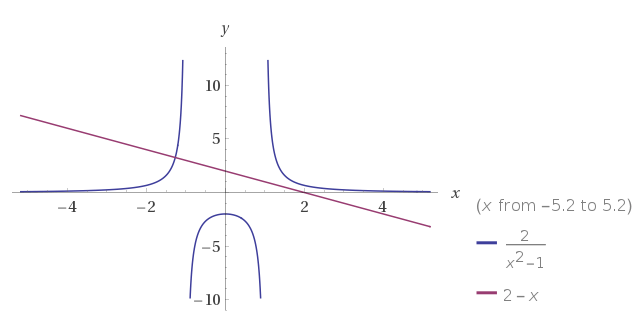
\includegraphics[width=14cm]{rozrahunkova_02/04_01.png}
  \label{fig:rr_02_04_01}
  \centering
\end{figure}

Судячи з графіку, задані лінії мають лише 1 точку пересічення $(\dfrac{2}{x^2-1} = 2-x)$, тому будемо вважати що таку площу знайти неможливо, оскільки вона нічим не обмежена.
 \\ \qquad \\
  % {\task{green}{В4 - РР2 - 04.02}} {\descr{Дослідити функцію на неперервність}}

$$
y=3^{\dfrac{2x}{3x+1}}
$$

Дослідимо функцію в точкі $-\dfrac{1}{3}$ де вона можливо має точку розриву.


$$
  \lim_{x \to -1/3 -0} 3^{\dfrac{2x}{3x+1}} \qquad \lim_{x \to (-1/3-0.001) -0} 3^{\dfrac{2x}{3x+1}} = \infty
$$

$$
  \lim_{x \to -1/3 +0} 3^{\dfrac{2x}{3x+1}} \qquad \lim_{x \to (-1/3+0.001) +0} 3^{\dfrac{2x}{3x+1}} = \infty
$$

\textbf{Висновок} - функція в точкі $-\dfrac{1}{3}$ тосить характер розриву \textbf{другого роду}, оскільки границі функції зліва та зправа прямують у нескінченність.


\begin{figure}[h!]
  \centering
  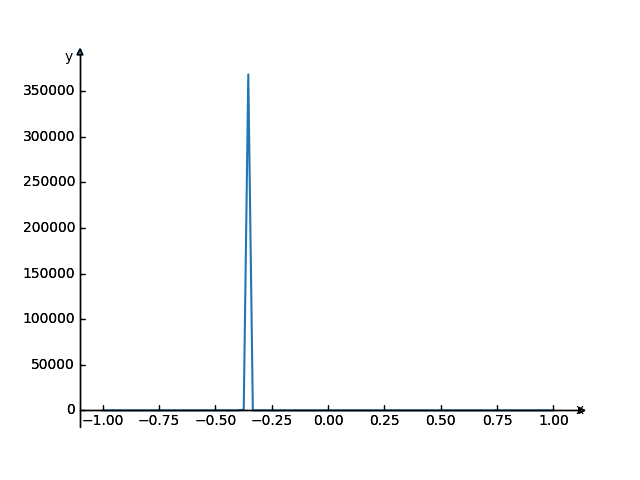
\includegraphics[width=14cm]{rozrahunkova_01/04_02.png}
  \caption{Графік функції}
  \label{fig:rr_01_40_02}
  \centering
\end{figure}
 \\ \qquad \\
  % {\task{green}{В4 - РР2 - 05.01}} {\descr[1]{Обчислити площу поверхні, одержаної при обертанні даннної кривої насколо осі OX}}

$$
  y = -\dfrac{1}{2}\ln{x}+\dfrac{x^2}{4} {\qquad} x \in [1;e]
$$

Для знаходження поверхні обертання використаємо наступну формулу

$$Q = 2\pi\int^b_a f(x) \sqrt{1+(f'(x))^2} \d{x} $$

$$
  2\pi \int^e_1 (-\dfrac{1}{2}\ln{x}+\dfrac{x^2}{4}) \sqrt{1+((\dfrac{x^2}{4}-\dfrac{1}{2}\ln{x})')^2} \d{x}
= 2\pi \int^e_1 \dfrac{1}{2} ( \dfrac{x^2}{2} - \ln{x} ) \sqrt{1+(\dfrac{x^2-1}{2x})^2} \d{x}
$$

$$
= \dfrac{2\pi}{2} ( \int^e_1  ( \dfrac{x^2}{2} - \ln{x} ) \sqrt{1+(\dfrac{x^2-1}{2x})^2} \d{x} )
= \pi \int^e_1  \dfrac{x^2}{2} \sqrt{1+(\dfrac{x^2-1}{2x})^2} \d{x} - \pi \int^e_1 \ln{x} \sqrt{1+(\dfrac{x^2-1}{2x})^2}
$$

$$
= \dfrac{\pi}{2} \int^e_1  x^2 \sqrt{\dfrac{4x^2+x^4-2x^2+1}{4x^2}} \d{x} - \pi \int^e_1 \ln{x} \sqrt{\dfrac{4x^2+x^4-2x^2+1}{4x^2}}\d{x}
$$

$$
= \dfrac{\pi}{2} \int^e_1  \dfrac{x^2}{2x} \sqrt{x^4+2x^2+1} \d{x} - \pi \int^e_1 \ln{x} \sqrt{\dfrac{x^2(x^2+2+\dfrac{1}{x^2})}{4x^2}}\d{x}
$$

$$
= \dfrac{\pi}{4} \int^e_1  x  \sqrt{(x^2+1)^2} \d{x} - \pi  \int^e_1 \dfrac{\ln{x}}{2} \sqrt{\dfrac{x^4+2x^2+1}{x^2}}\d{x}
$$

$$
= \dfrac{\pi}{4} \int^e_1  (x^3+x) \d{x} - \dfrac{\pi}{2}  \int^e_1 \ln{x} \sqrt{\dfrac{(x^2+1)^2}{x^2}}\d{x}
$$

$$
= \dfrac{\pi}{4} \int^e_1 x^3\d{x} + \dfrac{\pi}{4} \int^e_1 x \d{x} - \dfrac{\pi}{2}  \int^e_1  \dfrac{(x^2+1)\ln{x}}{x} \d{x}
$$

$$
= \dfrac{\pi}{4} \int^e_1 x^3\d{x} + \dfrac{\pi}{4} \int^e_1 x \d{x} - \dfrac{\pi}{2}( \int^e_1  \dfrac{x^2 \ln{x}}{x} \d{x} + \int^e_1 \dfrac{\ln{x}}{x} \d{x} )
$$


$$
= \dfrac{\pi}{4} \int^e_1 x^3\d{x} + \dfrac{\pi}{4} \int^e_1 x \d{x} - \dfrac{\pi}{2}\Bigg( \int^e_1  x\ln{x} \d{x} + \int^e_1 \dfrac{\ln{x}}{x} \d{x}
  \Bigg|
    \begin{array}{rlrlrlrl}
      u = & \ln{x} & x_1 = & e & y_1 = \ln{e} & = 1 \\
      u'= & \dfrac{1}{x} & x_0 = & 1 & y_0 = \ln{1} & = 0\\
      \end{array}
  \Bigg|
\Bigg)
$$

$$
= \dfrac{\pi}{4} \int^e_1 x^3\d{x} + \dfrac{\pi}{4} \int^e_1 x \d{x} - \dfrac{\pi}{2}( \int^e_1  x\ln{x} \d{x} + \int^1_0 u \d{u} )
$$

$$
= \dfrac{\pi}{4} \int^e_1 x^3\d{x} + \dfrac{\pi}{4} \int^e_1 x \d{x} - \dfrac{\pi}{2} \int^1_0 u \d{u}
 -  \dfrac{\pi}{2}\int^e_1  x\ln{x}  \d{x} \Bigg|
  \begin{array}{rlrl}
      u  =& \ln{x} & v  = & x^2/2 \\
      u' =& 1/x    & v' = & x \\
    \end{array}
\Bigg|
$$

$$
= \dfrac{\pi}{4} \int^e_1 x^3\d{x} + \dfrac{\pi}{4} \int^e_1 x \d{x} - \dfrac{\pi}{2} \int^1_0 u \d{u} -  \dfrac{\pi}{2} (\dfrac{x^2\ln{x}}{2} \Bigg|^e_1 - \int^e_1 \dfrac{1}{x} \dfrac{x^2}{2} \d{x} )
$$

$$
= \dfrac{\pi}{4} \int^e_1 x^3\d{x} + \dfrac{\pi}{4} \int^e_1 x \d{x} - \dfrac{\pi}{2} \int^1_0 u \d{u} -  \dfrac{\pi}{2} (\dfrac{x^2\ln{x}}{2} \Bigg|^e_1 - \dfrac{1}{2}\int^e_1 x\d{x} )
$$

Для більшої зручності порведемо обчислення визначених інтегралів окремо (формула вже завелика для копіювання навіть при наборі в LaTeX).

$$
1) \dfrac{\pi}{4} \int^e_1 x^3\d{x}
  = \dfrac{\pi}{4} \times \dfrac{x^4}{4}  \Bigg|^e_1
  = \dfrac{\pi}{16} (x^4) \Bigg|^e_1
  = \dfrac{\pi}{16} (e^4- 1^4)
  = \dfrac{\pi}{16} (e^4- 1)
$$

$$
2) \dfrac{\pi}{4} \int^e_1 x \d{x}
= \dfrac{\pi}{4} \times \dfrac{x^2}{2}  \Bigg|^e_1
= \dfrac{\pi}{8} (x^2) \Bigg|^e_1
= \dfrac{\pi}{8} (e^2 - 1^2)
= \dfrac{\pi}{8} (e^2 - 1)
$$


$$
3) - \dfrac{\pi}{2} \int^1_0 u \d{u} = - \dfrac{\pi}{4} (u^2)\Bigg|^1_0 = - \dfrac{\pi}{4} (1^2-0^2) = -\dfrac{\pi}{4}
$$

$$
4)  -  \dfrac{\pi}{2} \times \dfrac{x^2\ln{x}}{2} \Bigg|^e_1
= - \dfrac{\pi}{4} (e^2\ln{e}-1^2\ln{1})
= - \dfrac{\pi}{4} (e^2 \times 1 - 1^2 \times 0}) =
= - \dfrac{\pi e^2}{4}
$$

$$
5) - \dfrac{\pi}{2} \times -\dfrac{1}{2} \int^e_1 x\d{x}
= \dfrac{\pi}{4} \times \dfrac{x^2}{2}  \Bigg|^e_1
= \dfrac{\pi}{8} \times ( x^2 ) \Bigg|^e_1
= \dfrac{\pi}{8} \times ( e^2 - 1^2)
= \dfrac{\pi}{8} \times ( e^2 - 1)
$$

Залишилось лише просумувати отримані площі.

$$
\dfrac{\pi}{16} (e^4- 1) + \dfrac{\pi}{8} (e^2 - 1) -\dfrac{\pi}{4} - \dfrac{\pi e^2}{4} + \dfrac{\pi}{8} \times ( e^2 - 1)
= \dfrac{\pi}{16} (e^4- 1) + \dfrac{\pi}{4} (e^2 - 1) -\dfrac{\pi}{4} - \dfrac{\pi e^2}{4}
$$

$$
= \dfrac{\pi( (e^4-1) + 4(e^2-1) - 4 -4e^2)}{16}
= \dfrac{\pi( e^4-1 + 4e^2-4 - 4 -4e^2)}{16}
= \dfrac{\pi( e^4-9 ) }{16}
$$


$$
\boxed{ Q = \dfrac{\pi( e^4-9 ) }{16} }
$$
 \\ \qquad \\
  % {\task{green}{В4 - РР2 - 06.01}} {\descr[1]{Знайти обєм тіла, одержаного прі обертанні криволінійного заданого сектора навколо полярної осі:}}

$$
\rho = \alpha \sqrt{\cos{\varphi}},{\qquad} \varphi \in \Big[ 0; \dfrac{\pi}{2} \Big]
$$

Об'єм  тіла  отирманого обертанням в навколо полярної осі заданого двума поялрними координатами можна знайти за формулою
$$
V = \dfrac{2\pi}{3} \int_{\alpha}^{\beta} \rho^3\sin{\varphi} \d{\varphi}
$$

% http://energy.bmstu.ru/gormath/mathan2s/usint/UsingInt.htm#s121
$$
\dfrac{2\pi}{3} \int_0^{\dfrac{\pi}{2}} (a\sqrt{\cos{\varphi}})^3\sin{\varphi} \d{\varphi}
= \dfrac{2\pi}{3} \int_0^{\dfrac{\pi}{2}} a^3 \cos{\varphi}^{\dfrac{3}{2}}  \sin{\varphi} \d{\varphi}
\Bigg|
  \begin{array}{rl rl r}
     u =& \sin{\varphi} & \varphi_2 = & \dfrac{\pi}{2} & u_2 =   1  \\
    \d{u} =& \cos{\varphi} & \varphi_1 = & 0 & u_1 =   0 \\
  \end{array}
\Bigg| = \dfrac{2\pi a^4 }{3} \int^1_0 u^{\dfrac{3}{2}}\d{u}
$$

$$
= \dfrac{2\pi a^4 }{3} \int^1_0 u^{\dfrac{3}{2}}\d{u}
= \dfrac{a^4 \pi}{6} \dfrac{u^{\dfrac{5}{2}}}{\dfrac{5}{2}} \Bigg|_0^{1}
= \dfrac{a^4 \pi}{15} \sqrt{u^5} \Bigg|_0^{1}
= \dfrac{a^4 \pi}{15}
$$

$$
\boxed{V = \dfrac{a^4 \pi}{15} }
$$
 \\ \qquad \\
  % {\task{green}{В4 - РР2 - 07.01}} {\descr{Провести повне дослідження функції і побудувати графік}}

$$
y=\dfrac{2}{x^2+2x}
$$


1) $x \in (-\infty;-2)\cup(-2;0)\cup(0;+\infty)$

2) Графік не перетинає ось $x$.

3) Функція непарна оскільки

$$
  f(-x) = \dfrac{2}{(-x)^2+2(-x)} = \dfrac{2}{x^2-2x}
$$

4) Обидві точки -2 та 0 носить характер розриву другого роду оскільки вони прямують в безмежність.

$$
  \lim_{x \to -2 \ \pm0} \dfrac{2}{x^2+2x} = \mp \infty \qquad   \lim_{x \to 0 \ \pm0} \dfrac{2}{x^2+2x} = \pm \infty
$$

5) Похідна
$$
  y' = (\dfrac{2}{x^2+2x})'
     = \dfrac{2'(x^2+2x)-2(x^2+2x)'}{(x^2+2x)^2}
     = \dfrac{-4x-4}{(x^2+2x)^2}
$$

Функція не існує в точках $x=-2$ та $x=0$, а $x=-1$ є критичною (такою що є підозрілою на екстремум мінімум або максимум). На інтервалі $(-\infty;+\infty)$ матимемо:



\begin{center}
  \begin{tabular}{ | c | c | c | c | c | c | c | c | }
    \hline
      x     & (-\infty;-2) & -2 & (-2;-1) & -1 & (-1:0) & 0 &  (0; +\infty) \\
      \hline
      f'(x) &  + & не існує & + & 0  & -  & не існує & - \\
      \hline
      f(x)  & \nearrow  & не існує & \nearrow  & y_{max} = -2  & \searrow   & не існує & \searrow \\
    \hline
  \end{tabular}
\end{center}



6) Друга похідна

$$
  y'' = (\dfrac{-4x-4}{(x^2+2x)^2})'
  = \dfrac{(-4x-4)'(x^2+2x)^2 - (-4x-4)((x^2+2x)^2)' }{(x^2+2x)^4}
$$

$$
= \dfrac{-4(x^2+2x) + 4(2x+2)^2 }{(x^2+2x)^3}
= \dfrac{-4x^2-8x + 16x^2+32x+16 }{(x^2+2x)^3}
= \dfrac{12x^2+24x+16 }{(x^2+2x)^3}
$$

\begin{center}
  \begin{tabular}{ | c | c | c | c | c | c |  }
    \hline
    x & (-\infty;-2) & -2 & (-2:0) & 0 & (0:+\infty) \\
    \hline
    f"(x) &  + & не існує  & - & не існує & +  \\
    \hline
    f(x) &  \cup & не існує  & \cap & не існує & \cup \\
    \hline
  \end{tabular}
\end{center}

7) з пункта (4) випливає що фунція має вертикальні асимптоти в точках $x=-2$ та $x=0$.

Знаходимо горизонтальні асимптоти за формулами (через границі функції):
$$
  y = kx+b
$$

$$
  k = \lim_{x\to\infty} \dfrac{y(x)}{x}
    = \lim_{x\to\infty} \dfrac{2}{x(x^2+2x)}
    = \lim_{x\to\infty} \dfrac{2/x^2}{x(1+2/x)}
    = \dfrac{1}{\infty}
    = 0
$$

$$
  b = \lim_{x\to\infty} (y(x) - kx)
    = \lim_{x\to\infty} \dfrac{2}{x^2+2x}
    = \lim_{x\to\infty} \dfrac{2/x^2}{1+2/x}
    = \dfrac{0}{1}
    = 0
$$

8) Враховуючи висновки ослідження функції будуємо графік:

\begin{figure}[h!]
  \centering
  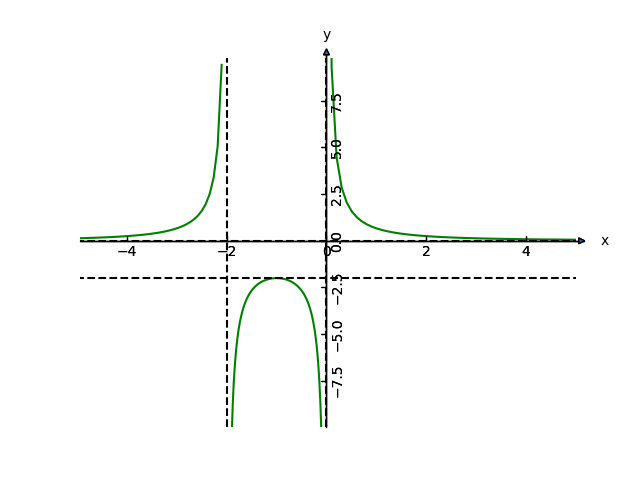
\includegraphics[width=14cm]{rozrahunkova_01/07_01.png}
  \caption{Графік функції $y=\dfrac{2}{x^2+2x}$ }
  \label{fig:rr_01_07_01}
  \centering
\end{figure}
 \\ \qquad \\

  % Ряди
  % {\task{orange}{В4 - РР3 - 01}} {\descr{Знайдіть n-y частинну суму $S_n$ і суму ряду $S$:}}

$$
  \sum_{n=1}^\infty \dfrac{n+1}{n^2(n+2)^2}
= \sum_{n=1}^\infty \dfrac{n+1}{n^4+4n^3+4n^2}
= \sum_{n=1}^\infty \dfrac{1}{4}\Big( \dfrac{1}{n^2} - \dfrac{1}{(n+2)^2} \Big)
$$

% маємо ряд діріхє, тоюто ряд зворотніх квадратів

\M{Спробуємо підставити числа і побачити закономірність}

$$
S_n = \dfrac{1}{4}\Big( \dfrac{1}{2^2} - \dfrac{1}{(2+2)^2} \Big) + \dfrac{1}{4}\Big( \dfrac{1}{3^2} - \dfrac{1}{(3+2)^2} \Big) \ldots + \dfrac{1}{4}\Big( \dfrac{1}{n^2} - \dfrac{1}{(n+2)^2} \Big)
$$
$$
= \dfrac{1}{4} \Bigg(
  \Big( \dfrac{1}{2^2} + \dfrac{1}{3^2} \ldots \dfrac{1}{n^2} \Big) -
  \Big( \dfrac{1}{(2+2)^2} + \dfrac{1}{(3+2)^2} \ldots \dfrac{1}{(n+2)^2} \Big)
  \Bigg)
$$
$$
= \dfrac{1}{4} \Bigg(
  \Big( \dfrac{1}{2^2} + \dfrac{1}{3^2} \ldots \dfrac{1}{n^2} \Big) -
  \Big( \dfrac{1}{4^2} + \dfrac{1}{5^2} \ldots \dfrac{1}{(n+2)^2} \Big)
  \Bigg)
$$

% http://math1.ru/education/num_series/sum_series1.html

\M{Тобто n-y частинну суму $S_n$ можна виразити як:}

$$
S_n = \sum_{n=1}^\infty \dfrac{1}{4}\Big( \dfrac{1}{n^2} - \dfrac{1}{(n+2)^2} \Big)
= \dfrac{1}{4} \Big( \sum_{n=1}^\infty  \dfrac{1}{n^2} - \sum_{n=3}^\infty \dfrac{1}{n^2}\Big)
= \dfrac{1}{4}  \sum_{n=1}^2  \dfrac{1}{n^2}
= \dfrac{1}{4} (\dfrac{1}{1}+\dfrac{1}{2^2}) = \boxed{\dfrac{5}{16}}
$$

\M{А сумою ряду, відповідно, буде}
$$
S
= \lim_{n \to \infty} \dfrac{n+1}{n^4+4n^3+4n^2}
= \lim_{n \to \infty}  \dfrac{\dfrac{1}{n^3}+\dfrac{1}{n^4}}{1+\dfrac{4}{n}+\dfrac{4}{n^2}  }
= \dfrac{0+0}{1+0+0  } \approx \boxed{0}
$$
 \\ \qquad \\
  % {\task{green}{В4 - РР3 - 03}} {\descr{Дослідіть ряд на збіжність:}}

$$
\sum_{n=2}^\infty \dfrac{\ln{n}}{n^2}
$$

$$
a_n = \dfrac{\ln{n}}{n^2}} < \dfrac{1}{n}  = b_n, \qquad n \geqslant 2
$$
За ознакою порівняння -  данний ряд є розбіжним, оскільки гармонічний ряд $\Sum{n=1}{\infty} \dfrac{1}{n}$ є розбіжним .
 \\ \qquad \\
  % {\task{orange}{В4 - РР3 - 04}} {\descr{Дослідіть ряд на збіжність:}}

$$
\sum_{n=1}^\infty \dfrac{n^2+1}{(3n)!}
$$

\M{Користуючись ознакою Даламбера, дослідимо ряд на збіжність:}

$$
 \lim_{n \to \infty} \dfrac{ \Big( \dfrac{(n+1)^2+1}{(3(n+1))!} \Big) }{ \Big( \dfrac{n^2+1}{(3n)!} \Big) }
=  \lim_{n \to \infty}  \dfrac{(n+1)^2+1}{(3(n+1))!} \times \dfrac{(3n)!}{n^2+1}
=  \lim_{n \to \infty}  \dfrac{(n+1)^2+1}{(3n+3)!} \times \dfrac{(3n)!}{n^2+1} =
$$
$$
=  \lim_{n \to \infty}  \dfrac{(n+1)^2+1}{(3n+3)!} \times \dfrac{(3n)!}{n^2+1}
= \lim_{n \to \infty}  \dfrac{n^2+2n+2}{(3n+3)(3n+2)(3n+1)(3n)!} \times \dfrac{(3n)!}{n^2+1}
$$

$$
= \lim_{n \to \infty}  \dfrac{n^2+2n+2}{(3n+3)(3n+2)(3n+1)(n^2+1)}
= \lim_{n \to \infty}  \dfrac{n^2+2 n+2}{27 n^5 + 54 n^4 + 60 n^3 + 60 n^2 + 33 n + 6}
$$

$$
= \lim_{n \to \infty}  \dfrac{ \dfrac{n^2}{n^5}+\dfrac{2n}{n^5}+\dfrac{2}{n^5}}{\dfrac{27 n^5}{n^5} + \dfrac{54 n^4}{n^5} + \dfrac{60 n^3}{n^5} + \dfrac{60 n^2}{n^5} + \dfrac{33 n}{n^5} + \dfrac{6}{n^5}}
= \lim_{n \to \infty}  \dfrac{ \dfrac{1}{n^3}^{\to0}+\dfrac{2}{n^4}^{\to0}+\dfrac{2}{n^5}^{\to0}}{27 + \dfrac{54}{n}^{\to0} + \dfrac{60}{n^2}^{\to0} + \dfrac{60}{n^3}^{\to0} + \dfrac{33}{n^4}^{\to0} + \dfrac{6}{n^5}^{\to0}} =
$$

$$
= \dfrac{ 0 + 0 + 0}{27 + 0 + 0 + 0 + 0 + 0 } \approx  \boxed{0} < 1
$$

\M{А отже ряд є збіжним за ознакою Даламбера:}
 \\ \qquad \\
  % {\task{green}{В4 - РР3 - 05}} {\descr{Дослідіть ряд на збіжність:}}

$$
\sum_{n=1}^\infty \Big(\dfrac{3n}{5n+1}\Big)^n
\Rightarrow
  \lim_{n \to \infty} \sqrt[n]{ \Big(\dfrac{3n}{5n+1}\Big)^n }
= \lim_{n \to \infty} \dfrac{3n}{5n+1}
= \lim_{n \to \infty} \dfrac{3}{5+1/n}
= \dfrac{3}{5+0}
= \dfrac{3}{5}
$$

\begin{center}Ряд є збіжним за ознакою Коші.\end{center}
 \\ \qquad \\
  % {\task{gray}{В4 - РР3 - 06}} {\descr{Дослідіть ряд на збіжність:}}

$$
\sum_{n=1}^\infty \dfrac{e^{1/n}-1}{\ln^2{3n}}
$$

$$
\lim_{n \to \infty} \dfrac{e^{1/n}-1}{\ln^2{3n}}
= \dfrac{\Lim{n \to \infty} e^{1/n}-1 }{\Lim{n \to \infty} \ln^2{3n}}
= \dfrac{\Lim{n \to \infty} e^{1/n}- \Lim{n \to \infty} 1  }{\Lim{n \to \infty} \ln^2{3n}} = \dfrac{1-1}{\infty} \approx 0
$$

\M{Що нe доводить  ні розбіжність, ні збіжність, але вказує на потенційну збіжність ряду}

 Оскільки $\dfrac{1}{n} \to 0$ то ми можемо скористатись цим і замінити $e^{1/n}-1$ на $\dfrac{1}{n}$ (це все за допомогою еквівалетним нескінченно малим функціям).

$$
  \sum_{n=1}^\infty \dfrac{e^{1/n}-1}{\ln^2{3n}}
= \sum_{n=1}^\infty \dfrac{1}{n\ln^2{3n}}
$$

Спробуємо скористатись інтегральною ознакою для дослідження ряду на збіжність:

$$
  \int_{1}^\infty \dfrac{\d{x}}{x\ln^2{3x}}
= \lim_{b \to \infty} \int^{+\infty}_1 \dfrac{\d{x}}{x\ln^2{3x}}
= - \lim_{b \to \infty} \dfrac{1}{\ln{3x}} \Bigg|^b_1
= - \lim_{b \to \infty} \dfrac{1}{\ln{3 \cdot \infty }} - \dfrac{1}{\ln{3}}
= - \Big( \dfrac{1}{\ln{3 \cdot \infty }} - \dfrac{1}{\ln{3}} \Big)
$$

$$
= - \Big( 0 - \dfrac{1}{\ln{3}} \Big) = \boxed{\dfrac{1}{\ln{3}}}
$$

\M{А отже ряд збігається за інтегральною ознакою}

% http://math1.ru/education/num_series/comp_test3.html
 \\ \qquad \\
  {\task{gray}{В4 - РР3 - 07}} {\descr{Дослідіть ряд на абсолютну або умовну збіжність:}}

$$
\sum_{n=1}^\infty (-1)^{n} {\cos{\dfrac{\pi}{4n+1}}}
$$

1) Знайдемо границю

% https://uk.wikipedia.org/wiki/%D0%94%D0%B8%D1%84%D0%B5%D1%80%D0%B5%D0%BD%D1%86%D1%96%D1%8E%D0%B2%D0%B0%D0%BD%D0%BD%D1%8F_%D1%81%D0%BA%D0%BB%D0%B0%D0%B4%D0%BD%D0%BE%D1%97_%D1%84%D1%83%D0%BD%D0%BA%D1%86%D1%96%D1%97

$$
\lim_{n \to \infty} \cos{\dfrac{\pi}{4n+1}}
= \cos( \lim_{n \to \infty} \dfrac{\pi}{4n+1} )
= \cos(\pi \cdot \lim_{n \to \infty} \dfrac{1}{4n+1} )
= \cos(\pi \cdot 0 ) = \cos {0} = 1
$$

\M{Оскільки границя не дорівнює нулю, ряд розходиться за необхідною ознакою.}
 \\ \qquad \\
  % {\task{gray}{В4 - РР3 - 08}} {\descr{Знайдіть наближено суму ряду з точністю \varepsilon}}

$$
  \sum_{n=1}^\infty \dfrac{(-1)^{n+1}}{(n+2)^{2n}}, \qquad \varepsilon = 0,001
$$

\begin{enumerate}
  \item  Знайдемо чому дорівнює границя:
         $$ \lim_{n \to \infty } \dfrac{1}{(n+2)^{2n}} \approx 0 $$

 \item Спробуємо використати ознаку Діріхлє для доведення збіжності знакозмінного ряду:

  $$
    \lim_{n \to \infty} \sqrt[n]{(\dfrac{1}{n+2})^{2n}}
  = \lim_{n \to \infty} \dfrac{1}{(n+2)^2}
  = \dfrac{1}{(\infty+2)^2}\approx 0 \Rightarrow {\text{ 0 < 1, тобто ряд збіжний}}
  $$

  \item Перевіримо ряд на ознаки ряду Лейбніца:
    \begin{itemize}
        \item Ряд задовільняє першу умову оскільки ряд є спадаючим (починаючи з n > 1).
        \item Як вже визначено в пункті 1. границя $u_n$ приблизно дорівнює нулю.
      \end{itemize}

\end{enumerate}

З чого можна зробити висновок що данний ряд є рядом Лейбніца.

Абсолютна похибка від заміни його суми ряду його n-ою чистиною сумою не перевищує модуля першого з його членів, що видкривається:

$$
\Big| r_n \Big| = \Big| S-S_n \Big| \leqslant \Big| u_{n+1} \Big| \leqslant \varepsilon
$$

\M{Підбираємо значення $n$, для якого виконується рівння}

$$\Big( \dfrac{1}{((n+1)+2)^{2n+1}} \Big) \leqslant 0.001 \Rightarrow n = \Boxed{2} \rightarrow \dfrac{1}{((2+1)+2)^2(2\cdot(2+1))} < 0.001 $$

Тому сума перших двох членів ряду дасть нам суму ряду з точністю $\varepsilon = 0.001$ :

$$
  S \approx = \dfrac{1}{3^2} + \dfrac{1}{4^4} = \boxed{0.1151}
$$
 \\ \qquad \\
  % {\task{gray}{В4 - РР3 - 11}} Знайдіть інтервал збіжності степеневого ряду

$$
  \sum_{n=1}^\infty \dfrac{(n+4)}{2^n(n^2+1)}(x-2)^n
$$

% https://math.semestr.ru/math/convergence.php

За допомогою ознаки Даламбера значення при якому ряд сходиться по модулю:

$$
\lim_{n \to \infty} \bigg| \dfrac{u_{n+1}}{u_n} \bigg|
= \lim_{n \to \infty} \bigg| \dfrac{((n+1)+4)(x-2)^{n+1}}{2^{n+1}((n+1)^2+1)} : \dfrac{(n+4)(x-2)^n}{2^n(n^2+1)} \bigg| =
$$

$$
= \lim_{n \to \infty} \bigg| \dfrac{((n+1)+4)(x-2)^{n+1}}{2^{n+1}((n+1)^2+1)} \times \dfrac{2^n(n^2+1)}{(n+4)(x-2)^n} \bigg|=
$$

$$
= \dfrac{|x-2|}{2} \lim_{n \to \infty}  \bigg| \dfrac{(n+5)}{((n+1)^2+1)} \times \dfrac{(n^2+1)}{(n+4)} \bigg|
= \dfrac{|x-2|}{2} \lim_{n \to \infty}  \bigg| \dfrac{n+5}{n^2+2n+3} \times \dfrac{n^2+1}{n+4} \bigg|
$$

$$
= \dfrac{|x-2|}{2} \lim_{n \to \infty}  \bigg| \dfrac{n^3+5n^2+n+5}{(n^3+2n^2+3n)+(4n^2+8n+12)} \bigg|
= \dfrac{|x-2|}{2} \lim_{n \to \infty}  \bigg| \dfrac{n^3+5n^2+n+5}{n^3+6n^2+11n+12} \bigg| =
$$

$$
= \dfrac{|x-2|}{2} \lim_{n \to \infty}  \bigg| \dfrac{1+\dfrac{5}{n}+\dfrac{1}{n^2}+\dfrac{5}{n^3}}{1+\dfrac{6}{n}+\dfrac{11}{n^2}+\dfrac{12}{n^3} } \bigg|
= \dfrac{|x-2|}{2} \times \dfrac{1+0+0+0}{1+0+0+0} = \dfrac{|x-2|}{2}
$$

\M{Данний ряд буде сходитись при $\dfrac{|x-2|}{2} <1$ тому визначимо інтервал збіжності ряду:}


$$
\dfrac{|x-2|}{2} <1
\Rightarrow
|x-2| < 2
\Rightarrow
-2 < x-2 < 2
\Rightarrow
-2 + 2 < x-2+2 < 2+2
\Rightarrow
0 < x < 4
$$

\M{Тобто ряд збіжний на інтервалі (0:4).}

В точці $x=0$ числовий ряд $\Sum{n=1}{\infty} \dfrac{(-1)^n \cdot 2^n \cdot  (n+4)}{2^n \cdot(n^2+1)} = \Sum{n=1}{\infty} \dfrac{(-1)^n \cdot   (n+4)}{ n^2+1} $  збіжний абсолютно.

В точці $x=4$ числовий ряд $\Sum{n=1}{\infty} \dfrac{ 2^n \cdot  (n+4)}{2^n \cdot(n^2+1)} = \Sum{n=1}{\infty} \dfrac{ n+4}{ n^2+1} $ збіжний абсолютно.

Таким чином ряд збігається на інтервалі $\boxed{[0:4]}$

% https://www.youtube.com/watch?v=pBiKBX29oto
 \\ \qquad \\
  % {\task{gray}{В4 - РР3 - 13}} Розвиньте функцію у ряд Тейлора за степенями $x-a$ та вкажіть область збіжності ряду:

$$
  f(x) = {\dfrac{1}{\sqrt[5]{1+x^2}}} = (1+x^2)^{-\frac{1}{5}}, \qquad a=0
$$

$$
{\text{ Формула ряду Тейлора }}\sum_{n=0}^\infty \dfrac{f^{(n)}(a)}{n!}(x-a)^n
$$

\M{Як ми бачимо ми маємо справу з біномінальним рядом (за умови що ми підставимо $x$ як $x^2$), що у точці $a=0$ перетворєються у ряд Маклорена:}

$$
{\text{ Формула ряду Маклорена }}\sum_{n=0}^\infty \dfrac{f^{(n)}(a)}{n!}x^n
$$

\M{Біномінальний ряд}

$$
(1+x)^{\alpha} = 1+\alpha x + \dfrac{\alpha(\alpha-1)}{2!}x^2 + \dfrac{\alpha(\alpha-1)(\alpha-2)}{3!}x^3 +\ldots + \dfrac{\alpha(\alpha-1)(\alpha-2)}{n!}x^3
$$


$$
(1+x^2)^{-\frac{1}{5}} = 1
  - \dfrac{ \dfrac{x^2}{5} }{ 1!}
  + \dfrac{ \Bigg( -\dfrac{1}{5} \times -\dfrac{6}{5} \Bigg) x^4}{2!}
  + \dfrac{ \Bigg( -\dfrac{1}{5} \times -\dfrac{6}{5} \times -\dfrac{11}{5} \Bigg) x^6} {3!}
  \ldots
  + \dfrac{ \Bigg( \Prod{k=0}{n-1} \big(-\dfrac{1-k}{5}\big) \Bigg) x^{2n} }{n!}
$$

\M{Область збіжності ряду визначаємо із нерівності $|x^2| < 1 \Rightarrow |x| < 1$}

%
% Цм розрахунки була зроблені до того як япроситав пор узагальнення біномінального ряду
%
%
% %
% \M{Знайдемо кілька перших похідних функції:}
% $$
% \begin{array}{lllll}
% f(x)  = & (1+x^2)^{-\frac{1}{5}} & f(0) &=& 1 \\
% \\
% f(x)' = & -\dfrac{2x}{5(1+x^2)^{\frac{6}{5}}} & f(0)' &=& \dfrac{0}{5} =  0 \\
% \\
% f(x)'' = & \dfrac{2(7x^2-5)}{25(1+x^2)^{\frac{11}{5}}} & f(0)'' &=&-\dfrac{10}{25}=-\dfrac{2}{5}\\
% \\
% f(x)''' = & \dfrac{24x(7x^2-15)}{125(1+x^2)^{\frac{16}{5}}} & f(0)''' &=& \dfrac{0}{125}  = 0\\
% \\
% f(x)'''' = & \dfrac{24(119x^4-510x^2+75)}{625(1+x^2)^{\frac{21}{5}}} & f(0)''' &=& \dfrac{1800}{625}  = \dfrac{72}{25} \\
% \\
% f(x)''''' = & \dfrac{528x(119x^4-850x^2+375)}{3125(1+x^2)^{\frac{26}{5}}} & f(0)''''' &=& \dfrac{0}{3125}  = 0\\
% \end{array}
% $$

% похідна третього і більшх порядків була отримана за допомогою сервісу
% wolfram alpha
%
% 1 = D[  -2x/(5(1 + x^2)^(6/5)), x]
% 2 = D[  2(7x^2-5) /( 25(1+x^2)^(11/5) ), x]
% 3 = D[  24x(7x^2-15) /( 125(1+x^2)^(16/5) ), x]
% 4 = D[  24(119x^4-510x^2+75) /( 625(1+x^2)^(21/5) ), x]
% 5 = D[  528x(119x^4-850x^2+375) /( 3125(1+x^2)^(26/5) ), x]

% \M{Оскільки $a=0$, наш ряд Тейлора перетворюється у ряд Маклорена.}
%
% \M{Ряд Маклорена}
%
% $$
%  1 + \dfrac{0}{1!}x - \dfrac{2}{5 \times 2!} x^2 + \dfrac{0}{3!}x^3 + \dfrac{72}{25 \times 4!}x^4 + \dfrac{0}{5!}x^5 \ldots + \dfrac{f^{(n)}(0)}{n!}x^n
%  = 1 + 0 - \dfrac{2}{5}x^2 + 0 + \dfrac{3}{25}x^4 + 0 + \ldots + \dfrac{f^{(n)}(0)}{n!}x^n
% $$
%
% \M{Як бачимо, ми маємо справу з біномінальним рядом:}

% https://www.youtube.com/watch?v=ePx71bN9TqM
% похідна n ного порядку


% Область збіжності https://ru.wikipedia.org/wiki/%D0%A0%D1%8F%D0%B4_%D0%A2%D0%B5%D0%B9%D0%BB%D0%BE%D1%80%D0%B0#%D0%9E%D0%B1%D0%BB%D0%B0%D1%81%D1%82%D1%8C_%D1%81%D1%85%D0%BE%D0%B4%D0%B8%D0%BC%D0%BE%D1%81%D1%82%D0%B8_%D1%80%D1%8F%D0%B4%D0%B0_%D0%A2%D0%B5%D0%B9%D0%BB%D0%BE%D1%80%D0%B0
 \\ \qquad \\
  % {\task{gray}{В4 - РР3 - 14}} Застосовуючи відповідні степеневі ряди, обчисліть з точністю $\varepsilon$ значення функції

$$
  \lg 3, {\qquad}e=10^{-4}
$$

Застосовуючи властивості логарифмів виведемо натуральний логарифм через десятичний

$$
\boxed{ \log_{a} x = \ln{x} \times \log_{a} e }
\Rightarrow
\boxed{ \lg {n} = \log_{10} {n} = \ln{n} \times \log_{10} e }
\Rightarrow
\boxed{ \lg {3} = \ln {3} \times \lg e } {\text{ де }} {\lg e = 0.43429448}
$$

\M{Таким чином ми можемо скористатись рядом для визначення функції $\lg 3$:}

$$
\ln{\Bigg( \dfrac{1+x}{1-x} \Bigg)}
= 2\Bigg( x + \dfrac{x^3}{3} + \dfrac{x^5}{5} + \dfrac{x^7}{7} \ldots + \dfrac{x^{2n-1}}{2n-1} \Bigg)
$$

$$
\dfrac{1+x}{1-x} = 3 \Rightarrow x = \dfrac{1}{2}
$$

\M{тобто:}

$$
\ln{3} = 2 \Bigg( \dfrac{1}{2} + \dfrac{1}{3 \cdot 2^3 } + \dfrac{1}{5 \cdot 2^5} + \dfrac{1}{7 \cdot 2^7 }  + \ldots + \dfrac{1}{(2n-1) \cdot 2^{2n-1}}\Bigg).
$$

\M{Число членів ряду $n$ визначається нерівністю:}

$$
\bigg | r_n\Big( \dfrac{1}{2} \Big) \bigg | \leqslant \dfrac{2}{2^{2n-1} (2n-1)(1-\dfrac{1}{2^2})}  < 10^{-4}
$$

\M{ця нерівність задовольняється при $n=6$. Таким чином:}

$$
\ln{3} \approx 2 \Big(
\dfrac{1}{\cdot 2 } + \dfrac{1}{3 \cdot 2^3 } +
 \dfrac{1}{5 \cdot 2^5 } + \dfrac{1}{7 \cdot 2^7 } +
 \dfrac{1}{9 \cdot 2^9 } + \dfrac{1}{11 \cdot 2^{11} }
\Big) = 1.0985882823773445
$$

\M{І фінально підставивши модуль переходу отримаємо значення функції $\lg{3}$ з точністю $10^{-4}$:}
$$\ln{3} \cdot \lg e = 1.0985882823773445 \cdot 0.43429448 = \boxed{ 0.4771 }$$

\M{\scriptsize{Рахувалось в мові програмування Python}}
 \\ \qquad \\
  % {\task{gray}{В4 - РР3 - 15}} Обчисліть з точністю до $\varepsilon=10^{-3}$ інтерграл:

$$
  \int_{3}^{\infty} \dfrac{\d{x}}{1+x^4}
$$

Оскільки $x \geqslant 3 $ то розвинемо підінтегральну функцію за степенями \dfrac{1}{x}:

$$
\dfrac{1}{1+x^4}
= \dfrac{1}{x^4} \cdot \dfrac{1}{1+\dfrac{1}{x^4}}
= \dfrac{1}{x^4} \Big( 1 - \dfrac{1}{x^4} + \dfrac{1}{x^8} - \ldots + (-1)^n\dfrac{1}{x^{4n}}\Big)
= \dfrac{1}{x^4} - \dfrac{1}{x^8} + \dfrac{1}{x^4} - \ldots + (-1)^n\dfrac{1}{x^{4(x+1)}}+\ldots, |x| > 1
$$

\M{Проінтегруємо цей ряд на порміжку $[3;+\infty)$ який належить області збіжності ряду.}

$$
\int^\infty_{3} \dfrac{\d{x}}{1+x^4}
= \sum^\infty_{n=0} \int^\infty_{3} (-1)^n\dfrac{1}{x^{4x+4}} \d{x}
= \sum^\infty_{n=0}(-1)^{n+1} \dfrac{1}{(4n+3)x^{4n+3}} \Bigg|^\infty_{3}
$$
$$
= \sum^\infty_{n=0}(-1)^{n+1} \dfrac{1}{(4n+3)} \Bigg( \dfrac{1}{\infty^{4n+3}} - \dfrac{1}{3^{4n+3}} \Bigg) = \sum^\infty_{n=0}(-1)^n \dfrac{1}{(4n+3)3^{4n+3}}
$$

\M{Знаходимо кількість членів n для яких виконується рівність}

$$\Big|r_n\Big| \leqslant \dfrac{1}{(4n+3)3^{4n+3}} < 10^{-3} \rightarrow n > 1$$

\M{тому:}
$$
  \int_{3}^{\infty} \dfrac{\d{x}}{1+x^4} \approx \dfrac{1}{(0+3)3^{0+3}} = \dfrac{1}{3^4} = \boxed{0.012}
$$
 \\ \qquad \\
\end{document}
%
%
%
